%!TEX root = hulk.tex
%!TeX TS-program = pdflatex
%!TeX encoding = UTF-8 Unicode
%!TeX spellcheck = en-US
%!BIB TS-program = bibtex
% -*- coding: UTF-8; -*-
% vim: set fenc=utf-8
% https://github.com/bicv/Perrinet2015BICV_sparse/blob/master/sparse.tex
% TODO : change notation for x = A @ y
%%%%%%%%%%%%%%%%%%%%%%%%%%%%%%%%%%%%%%%%%%%%%%%%%%%%%%%%%%%%%%%%%%%%%
%%%%%%%%%%%%%%%%%%%%%%%%%%%%%%%%%%%%%%%%%%%%%%%%%%%%%%%%%%%%%%%%%%%%%
\documentclass[letterpaper,final,conference,10pt]{IEEEtran}
%============ common ===================
%\usepackage[utf8]{luainputenc}
%\usepackage[english]{babel}%
%%\usepackage{csquotes}%
%\usepackage[autostyle]{csquotes}
%%% Sans-serif Arial-like fonts
%\renewcommand{\rmdefault}{phv}
%\renewcommand{\sfdefault}{phv}
%   \usepackage{textcomp}
%   \usepackage{libertine}%[sb]
%   \usepackage[varqu,varl]{inconsolata}% sans serif typewriter
%   \usepackage[libertine,bigdelims,vvarbb]{newtxmath} % bb from STIX
%   \usepackage[cal=boondoxo]{mathalfa} % mathcal
%%   \useosf % osf for text, not math
%   \usepackage[supstfm=libertinesups,%
%    supscaled=1.2,%
%    raised=-.13em]{superiors}
%\usepackage[utf8]{inputenc} % allow utf-8 input
%\usepackage[T1]{fontenc}    % use 8-bit T1 fonts
%\usepackage{dsfont}
%\usepackage{hyperref}       % hyperlinks
% --------------------------------------------------------------------------
%                    METADATA
% --------------------------------------------------------------------------
\newcommand{\AuthorA}{Boutin}%
\newcommand{\FirstNameA}{Victor}%
\newcommand{\AuthorB}{Franciosini}%
\newcommand{\FirstNameB}{Angelo}%
\newcommand{\AuthorC}{Perrinet}%
\newcommand{\FirstNameC}{Laurent U}%
\newcommand{\Institute}{Institut Neurosciences Timone}%, Marseille, France}%\\ Aix Marseille Univ, CNRS}%
\newcommand{\Organism}{Aix Marseille Université, CNRS}%
\newcommand{\Address}{27, Bd. Jean Moulin, 13385 Marseille Cedex 5, France}%
\newcommand{\EmailA}{victor.boutin@univ-amu.fr}%
\newcommand{\EmailB}{angelo.franciosini@univ-amu.fr}%
\newcommand{\EmailC}{laurent.perrinet@univ-amu.fr}%
\newcommand{\Website}{https://spikeai.github.io/}%
\newcommand{\WebsiteC}{https://spikeai.github.io/}%
\newcommand{\Title}{%
%alternatives: - Homeostasis is necessary for the unsupervised learning of orientation-selective cells
%# Homeostatic Unsupervised Learning of Kernels
%An adaptive homeostatic algorithm for the unsupervised learning of independent visual features
%A fast algorithm for unsupervised learning
An adaptive homeostatic algorithm for the unsupervised learning of visual features
}%
\newcommand{\Abstract}{ %  13 characters left
The formation of structure in the brain, that is, of the connections between cells within neural populations, is by large an unsupervised learning process: the emergence of this architecture is mostly self-organized. In the primary visual cortex of mammals, for example, one may observe during development the formation of cells selective to localized, oriented features. This leads to the development of a rough representation of contours of the retinal image in area V1. We modeled these mechanisms using sparse Hebbian learning algorithms. These algorithms alternate a coding step to encode the information with a learning step to find the proper encoder. A major difficulty is to deduce a good representation while knowing immature encoders, and to learn good encoders with a non-optimal representation. To address this problem, we propose to introduce a new regulation process between learning and coding, called homeostasis. It is compatible with a neuro-mimetic architecture and allows for the fast emergence of localized filters sensitive to orientation. The key to this algorithm lies in a simple adaptation mechanism based on non-linear functions that reconciles the antagonistic processes that occur at the coding and learning time scales. We tested this unsupervised algorithm with this homeostasis rule for a range of learning algorithms coupled with different neural coding algorithms. In addition, we propose a simplification of this optimal homeostasis rule by implementing a simple heuristic on the probability of activation of neurons. Compared to the optimal homeostasis rule, we show that this heuristic allows to implement a more rapid unsupervised learning algorithm while keeping a large part of its effectiveness. These results demonstrate the potential application of such a strategy in machine learning and we illustrate this with one result in a convolutional neural network.
}
\newcommand{\Keywords}{Vision, Sparseness, Computer vision, Unsupervised learning, Neuroscience}%
\newcommand{\SubjectAreas}{Sparse Coding, Unsupervised Learning, Natural Scene Statistics, Biologically Plausible Deep Networks, Visual Perception, Computer Vision}%
\newcommand{\Acknowledgments}{%
%This work was supported by XXXAFXXX and the Doc2Amu project which received funding from a co-fund with the European Union's Horizon 2020 research and innovation programme and the region Provence Alpes Cote d'Azur.
%
This research has received funding from the European Union’s Horizon 2020 research and innovation programme under the Marie Skłodowska-Curie grant agreement No713750. Also, it has been carried out with the financial support of the Regional Council of Provence-Alpes-Côte d’Azur and with the financial support of the A*MIDEX (n° ANR- 11-IDEX-0001-02), funded by the Investissements d'Avenir project funded by the French Government, managed by the French National Research Agency (ANR).
}
\newcommand{\Links}{%
\begin{itemize}
\item Correspondence and requests for materials should be addressed to LUP (email:\EmailC ).
\item Code and supplementary material available at \url{\WebsiteC/Publications/BoutinFranciosiniPerrinet18hulk}.
\end{itemize}
} %
\newcommand{\citep}[1]{\cite{#1}}
%\newcommand{\citet}[1]{(\textcite{#1})}
%%%%%%%%%%%%%%%%%%%%%%%%%%%%%%
%\usepackage[unicode,linkcolor=blue,citecolor=blue,filecolor=black,urlcolor=blue,pdfborder={0 0 0}]{hyperref}%
%\hypersetup{%
%pdftitle={\Title},%
%pdfauthor={Corrresponding author: \AuthorC < \EmailC > \Address - \WebsiteC },%
%pdfkeywords={\Keywords},%
%pdfsubject={\Acknowledgments}%
%}%
%\usepackage[utf8]{inputenc} % allow utf-8 input
%\usepackage[T1]{fontenc}    % use 8-bit T1 fonts
\usepackage{hyperref}       % hyperlinks
\usepackage{url}            % simple URL typesetting
\usepackage{booktabs}       % professional-quality tables
\usepackage{nicefrac}       % compact symbols for 1/2, etc.
\usepackage{microtype}      % microtypography

\usepackage[final]{pdfpages}
\newcommand{\printingPaperWidth}{216mm}
%\usepackage{xcolor}
\usepackage{amsmath,amssymb,amsfonts}
\usepackage{algpseudocode}
\usepackage{textcomp}
%\usepackage[dvipsnames]{xcolor}
\usepackage{xcolor}
% Optional math commands from https://github.com/goodfeli/dlbook_notation.
%%%%% NEW MATH DEFINITIONS %%%%%

\usepackage{amsmath,amsfonts,bm}

% Mark sections of captions for referring to divisions of figures
\newcommand{\figleft}{{\em (Left)}}
\newcommand{\figcenter}{{\em (Center)}}
\newcommand{\figright}{{\em (Right)}}
\newcommand{\figtop}{{\em (Top)}}
\newcommand{\figbottom}{{\em (Bottom)}}
\newcommand{\captiona}{{\em (a)}}
\newcommand{\captionb}{{\em (b)}}
\newcommand{\captionc}{{\em (c)}}
\newcommand{\captiond}{{\em (d)}}

% Highlight a newly defined term
\newcommand{\newterm}[1]{{\bf #1}}


% Figure reference, lower-case.
\def\figref#1{figure~\ref{#1}}
% Figure reference, capital. For start of sentence
\def\Figref#1{Figure~\ref{#1}}
\def\twofigref#1#2{figures \ref{#1} and \ref{#2}}
\def\quadfigref#1#2#3#4{figures \ref{#1}, \ref{#2}, \ref{#3} and \ref{#4}}
% Section reference, lower-case.
\def\secref#1{section~\ref{#1}}
% Section reference, capital.
\def\Secref#1{Section~\ref{#1}}
% Reference to two sections.
\def\twosecrefs#1#2{sections \ref{#1} and \ref{#2}}
% Reference to three sections.
\def\secrefs#1#2#3{sections \ref{#1}, \ref{#2} and \ref{#3}}
% Reference to an equation, lower-case.
\def\eqref#1{equation~\ref{#1}}
% Reference to an equation, upper case
\def\Eqref#1{Equation~\ref{#1}}
% A raw reference to an equation---avoid using if possible
\def\plaineqref#1{\ref{#1}}
% Reference to a chapter, lower-case.
\def\chapref#1{chapter~\ref{#1}}
% Reference to an equation, upper case.
\def\Chapref#1{Chapter~\ref{#1}}
% Reference to a range of chapters
\def\rangechapref#1#2{chapters\ref{#1}--\ref{#2}}
% Reference to an algorithm, lower-case.
\def\algref#1{algorithm~\ref{#1}}
% Reference to an algorithm, upper case.
\def\Algref#1{Algorithm~\ref{#1}}
\def\twoalgref#1#2{algorithms \ref{#1} and \ref{#2}}
\def\Twoalgref#1#2{Algorithms \ref{#1} and \ref{#2}}
% Reference to a part, lower case
\def\partref#1{part~\ref{#1}}
% Reference to a part, upper case
\def\Partref#1{Part~\ref{#1}}
\def\twopartref#1#2{parts \ref{#1} and \ref{#2}}

\def\ceil#1{\lceil #1 \rceil}
\def\floor#1{\lfloor #1 \rfloor}
\def\1{\bm{1}}
\newcommand{\train}{\mathcal{D}}
\newcommand{\valid}{\mathcal{D_{\mathrm{valid}}}}
\newcommand{\test}{\mathcal{D_{\mathrm{test}}}}

\def\eps{{\epsilon}}


% Random variables
\def\reta{{\textnormal{$\eta$}}}
\def\ra{{\textnormal{a}}}
\def\rb{{\textnormal{b}}}
\def\rc{{\textnormal{c}}}
\def\rd{{\textnormal{d}}}
\def\re{{\textnormal{e}}}
\def\rf{{\textnormal{f}}}
\def\rg{{\textnormal{g}}}
\def\rh{{\textnormal{h}}}
\def\ri{{\textnormal{i}}}
\def\rj{{\textnormal{j}}}
\def\rk{{\textnormal{k}}}
\def\rl{{\textnormal{l}}}
% rm is already a command, just don't name any random variables m
\def\rn{{\textnormal{n}}}
\def\ro{{\textnormal{o}}}
\def\rp{{\textnormal{p}}}
\def\rq{{\textnormal{q}}}
\def\rr{{\textnormal{r}}}
\def\rs{{\textnormal{s}}}
\def\rt{{\textnormal{t}}}
\def\ru{{\textnormal{u}}}
\def\rv{{\textnormal{v}}}
\def\rw{{\textnormal{w}}}
\def\rx{{\textnormal{x}}}
\def\ry{{\textnormal{y}}}
\def\rz{{\textnormal{z}}}

% Random vectors
\def\rvepsilon{{\mathbf{\epsilon}}}
\def\rvtheta{{\mathbf{\theta}}}
\def\rva{{\mathbf{a}}}
\def\rvb{{\mathbf{b}}}
\def\rvc{{\mathbf{c}}}
\def\rvd{{\mathbf{d}}}
\def\rve{{\mathbf{e}}}
\def\rvf{{\mathbf{f}}}
\def\rvg{{\mathbf{g}}}
\def\rvh{{\mathbf{h}}}
\def\rvu{{\mathbf{i}}}
\def\rvj{{\mathbf{j}}}
\def\rvk{{\mathbf{k}}}
\def\rvl{{\mathbf{l}}}
\def\rvm{{\mathbf{m}}}
\def\rvn{{\mathbf{n}}}
\def\rvo{{\mathbf{o}}}
\def\rvp{{\mathbf{p}}}
\def\rvq{{\mathbf{q}}}
\def\rvr{{\mathbf{r}}}
\def\rvs{{\mathbf{s}}}
\def\rvt{{\mathbf{t}}}
\def\rvu{{\mathbf{u}}}
\def\rvv{{\mathbf{v}}}
\def\rvw{{\mathbf{w}}}
\def\rvx{{\mathbf{x}}}
\def\rvy{{\mathbf{y}}}
\def\rvz{{\mathbf{z}}}

% Elements of random vectors
\def\erva{{\textnormal{a}}}
\def\ervb{{\textnormal{b}}}
\def\ervc{{\textnormal{c}}}
\def\ervd{{\textnormal{d}}}
\def\erve{{\textnormal{e}}}
\def\ervf{{\textnormal{f}}}
\def\ervg{{\textnormal{g}}}
\def\ervh{{\textnormal{h}}}
\def\ervi{{\textnormal{i}}}
\def\ervj{{\textnormal{j}}}
\def\ervk{{\textnormal{k}}}
\def\ervl{{\textnormal{l}}}
\def\ervm{{\textnormal{m}}}
\def\ervn{{\textnormal{n}}}
\def\ervo{{\textnormal{o}}}
\def\ervp{{\textnormal{p}}}
\def\ervq{{\textnormal{q}}}
\def\ervr{{\textnormal{r}}}
\def\ervs{{\textnormal{s}}}
\def\ervt{{\textnormal{t}}}
\def\ervu{{\textnormal{u}}}
\def\ervv{{\textnormal{v}}}
\def\ervw{{\textnormal{w}}}
\def\ervx{{\textnormal{x}}}
\def\ervy{{\textnormal{y}}}
\def\ervz{{\textnormal{z}}}

% Random matrices
\def\rmA{{\mathbf{A}}}
\def\rmB{{\mathbf{B}}}
\def\rmC{{\mathbf{C}}}
\def\rmD{{\mathbf{D}}}
\def\rmE{{\mathbf{E}}}
\def\rmF{{\mathbf{F}}}
\def\rmG{{\mathbf{G}}}
\def\rmH{{\mathbf{H}}}
\def\rmI{{\mathbf{I}}}
\def\rmJ{{\mathbf{J}}}
\def\rmK{{\mathbf{K}}}
\def\rmL{{\mathbf{L}}}
\def\rmM{{\mathbf{M}}}
\def\rmN{{\mathbf{N}}}
\def\rmO{{\mathbf{O}}}
\def\rmP{{\mathbf{P}}}
\def\rmQ{{\mathbf{Q}}}
\def\rmR{{\mathbf{R}}}
\def\rmS{{\mathbf{S}}}
\def\rmT{{\mathbf{T}}}
\def\rmU{{\mathbf{U}}}
\def\rmV{{\mathbf{V}}}
\def\rmW{{\mathbf{W}}}
\def\rmX{{\mathbf{X}}}
\def\rmY{{\mathbf{Y}}}
\def\rmZ{{\mathbf{Z}}}

% Elements of random matrices
\def\ermA{{\textnormal{A}}}
\def\ermB{{\textnormal{B}}}
\def\ermC{{\textnormal{C}}}
\def\ermD{{\textnormal{D}}}
\def\ermE{{\textnormal{E}}}
\def\ermF{{\textnormal{F}}}
\def\ermG{{\textnormal{G}}}
\def\ermH{{\textnormal{H}}}
\def\ermI{{\textnormal{I}}}
\def\ermJ{{\textnormal{J}}}
\def\ermK{{\textnormal{K}}}
\def\ermL{{\textnormal{L}}}
\def\ermM{{\textnormal{M}}}
\def\ermN{{\textnormal{N}}}
\def\ermO{{\textnormal{O}}}
\def\ermP{{\textnormal{P}}}
\def\ermQ{{\textnormal{Q}}}
\def\ermR{{\textnormal{R}}}
\def\ermS{{\textnormal{S}}}
\def\ermT{{\textnormal{T}}}
\def\ermU{{\textnormal{U}}}
\def\ermV{{\textnormal{V}}}
\def\ermW{{\textnormal{W}}}
\def\ermX{{\textnormal{X}}}
\def\ermY{{\textnormal{Y}}}
\def\ermZ{{\textnormal{Z}}}

% Vectors
\def\vzero{{\bm{0}}}
\def\vone{{\bm{1}}}
\def\vmu{{\bm{\mu}}}
\def\vtheta{{\bm{\theta}}}
\def\va{{\bm{a}}}
\def\vb{{\bm{b}}}
\def\vc{{\bm{c}}}
\def\vd{{\bm{d}}}
\def\ve{{\bm{e}}}
\def\vf{{\bm{f}}}
\def\vg{{\bm{g}}}
\def\vh{{\bm{h}}}
\def\vi{{\bm{i}}}
\def\vj{{\bm{j}}}
\def\vk{{\bm{k}}}
\def\vl{{\bm{l}}}
\def\vm{{\bm{m}}}
\def\vn{{\bm{n}}}
\def\vo{{\bm{o}}}
\def\vp{{\bm{p}}}
\def\vq{{\bm{q}}}
\def\vr{{\bm{r}}}
\def\vs{{\bm{s}}}
\def\vt{{\bm{t}}}
\def\vu{{\bm{u}}}
\def\vv{{\bm{v}}}
\def\vw{{\bm{w}}}
\def\vx{{\bm{x}}}
\def\vy{{\bm{y}}}
\def\vz{{\bm{z}}}

% Elements of vectors
\def\evalpha{{\alpha}}
\def\evbeta{{\beta}}
\def\evepsilon{{\epsilon}}
\def\evlambda{{\lambda}}
\def\evomega{{\omega}}
\def\evmu{{\mu}}
\def\evpsi{{\psi}}
\def\evsigma{{\sigma}}
\def\evtheta{{\theta}}
\def\eva{{a}}
\def\evb{{b}}
\def\evc{{c}}
\def\evd{{d}}
\def\eve{{e}}
\def\evf{{f}}
\def\evg{{g}}
\def\evh{{h}}
\def\evi{{i}}
\def\evj{{j}}
\def\evk{{k}}
\def\evl{{l}}
\def\evm{{m}}
\def\evn{{n}}
\def\evo{{o}}
\def\evp{{p}}
\def\evq{{q}}
\def\evr{{r}}
\def\evs{{s}}
\def\evt{{t}}
\def\evu{{u}}
\def\evv{{v}}
\def\evw{{w}}
\def\evx{{x}}
\def\evy{{y}}
\def\evz{{z}}

% Matrix
\def\mA{{\bm{A}}}
\def\mB{{\bm{B}}}
\def\mC{{\bm{C}}}
\def\mD{{\bm{D}}}
\def\mE{{\bm{E}}}
\def\mF{{\bm{F}}}
\def\mG{{\bm{G}}}
\def\mH{{\bm{H}}}
\def\mI{{\bm{I}}}
\def\mJ{{\bm{J}}}
\def\mK{{\bm{K}}}
\def\mL{{\bm{L}}}
\def\mM{{\bm{M}}}
\def\mN{{\bm{N}}}
\def\mO{{\bm{O}}}
\def\mP{{\bm{P}}}
\def\mQ{{\bm{Q}}}
\def\mR{{\bm{R}}}
\def\mS{{\bm{S}}}
\def\mT{{\bm{T}}}
\def\mU{{\bm{U}}}
\def\mV{{\bm{V}}}
\def\mW{{\bm{W}}}
\def\mX{{\bm{X}}}
\def\mY{{\bm{Y}}}
\def\mZ{{\bm{Z}}}
\def\mBeta{{\bm{\beta}}}
\def\mPhi{{\bm{\Phi}}}
\def\mLambda{{\bm{\Lambda}}}
\def\mSigma{{\bm{\Sigma}}}

% Tensor
\DeclareMathAlphabet{\mathsfit}{\encodingdefault}{\sfdefault}{m}{sl}
\SetMathAlphabet{\mathsfit}{bold}{\encodingdefault}{\sfdefault}{bx}{n}
\newcommand{\tens}[1]{\bm{\mathsfit{#1}}}
\def\tA{{\tens{A}}}
\def\tB{{\tens{B}}}
\def\tC{{\tens{C}}}
\def\tD{{\tens{D}}}
\def\tE{{\tens{E}}}
\def\tF{{\tens{F}}}
\def\tG{{\tens{G}}}
\def\tH{{\tens{H}}}
\def\tI{{\tens{I}}}
\def\tJ{{\tens{J}}}
\def\tK{{\tens{K}}}
\def\tL{{\tens{L}}}
\def\tM{{\tens{M}}}
\def\tN{{\tens{N}}}
\def\tO{{\tens{O}}}
\def\tP{{\tens{P}}}
\def\tQ{{\tens{Q}}}
\def\tR{{\tens{R}}}
\def\tS{{\tens{S}}}
\def\tT{{\tens{T}}}
\def\tU{{\tens{U}}}
\def\tV{{\tens{V}}}
\def\tW{{\tens{W}}}
\def\tX{{\tens{X}}}
\def\tY{{\tens{Y}}}
\def\tZ{{\tens{Z}}}


% Graph
\def\gA{{\mathcal{A}}}
\def\gB{{\mathcal{B}}}
\def\gC{{\mathcal{C}}}
\def\gD{{\mathcal{D}}}
\def\gE{{\mathcal{E}}}
\def\gF{{\mathcal{F}}}
\def\gG{{\mathcal{G}}}
\def\gH{{\mathcal{H}}}
\def\gI{{\mathcal{I}}}
\def\gJ{{\mathcal{J}}}
\def\gK{{\mathcal{K}}}
\def\gL{{\mathcal{L}}}
\def\gM{{\mathcal{M}}}
\def\gN{{\mathcal{N}}}
\def\gO{{\mathcal{O}}}
\def\gP{{\mathcal{P}}}
\def\gQ{{\mathcal{Q}}}
\def\gR{{\mathcal{R}}}
\def\gS{{\mathcal{S}}}
\def\gT{{\mathcal{T}}}
\def\gU{{\mathcal{U}}}
\def\gV{{\mathcal{V}}}
\def\gW{{\mathcal{W}}}
\def\gX{{\mathcal{X}}}
\def\gY{{\mathcal{Y}}}
\def\gZ{{\mathcal{Z}}}

% Sets
\def\sA{{\mathbb{A}}}
\def\sB{{\mathbb{B}}}
\def\sC{{\mathbb{C}}}
\def\sD{{\mathbb{D}}}
% Don't use a set called E, because this would be the same as our symbol
% for expectation.
\def\sF{{\mathbb{F}}}
\def\sG{{\mathbb{G}}}
\def\sH{{\mathbb{H}}}
\def\sI{{\mathbb{I}}}
\def\sJ{{\mathbb{J}}}
\def\sK{{\mathbb{K}}}
\def\sL{{\mathbb{L}}}
\def\sM{{\mathbb{M}}}
\def\sN{{\mathbb{N}}}
\def\sO{{\mathbb{O}}}
\def\sP{{\mathbb{P}}}
\def\sQ{{\mathbb{Q}}}
\def\sR{{\mathbb{R}}}
\def\sS{{\mathbb{S}}}
\def\sT{{\mathbb{T}}}
\def\sU{{\mathbb{U}}}
\def\sV{{\mathbb{V}}}
\def\sW{{\mathbb{W}}}
\def\sX{{\mathbb{X}}}
\def\sY{{\mathbb{Y}}}
\def\sZ{{\mathbb{Z}}}

% Entries of a matrix
\def\emLambda{{\Lambda}}
\def\emA{{A}}
\def\emB{{B}}
\def\emC{{C}}
\def\emD{{D}}
\def\emE{{E}}
\def\emF{{F}}
\def\emG{{G}}
\def\emH{{H}}
\def\emI{{I}}
\def\emJ{{J}}
\def\emK{{K}}
\def\emL{{L}}
\def\emM{{M}}
\def\emN{{N}}
\def\emO{{O}}
\def\emP{{P}}
\def\emQ{{Q}}
\def\emR{{R}}
\def\emS{{S}}
\def\emT{{T}}
\def\emU{{U}}
\def\emV{{V}}
\def\emW{{W}}
\def\emX{{X}}
\def\emY{{Y}}
\def\emZ{{Z}}
\def\emSigma{{\Sigma}}

% entries of a tensor
% Same font as tensor, without \bm wrapper
\newcommand{\etens}[1]{\mathsfit{#1}}
\def\etLambda{{\etens{\Lambda}}}
\def\etA{{\etens{A}}}
\def\etB{{\etens{B}}}
\def\etC{{\etens{C}}}
\def\etD{{\etens{D}}}
\def\etE{{\etens{E}}}
\def\etF{{\etens{F}}}
\def\etG{{\etens{G}}}
\def\etH{{\etens{H}}}
\def\etI{{\etens{I}}}
\def\etJ{{\etens{J}}}
\def\etK{{\etens{K}}}
\def\etL{{\etens{L}}}
\def\etM{{\etens{M}}}
\def\etN{{\etens{N}}}
\def\etO{{\etens{O}}}
\def\etP{{\etens{P}}}
\def\etQ{{\etens{Q}}}
\def\etR{{\etens{R}}}
\def\etS{{\etens{S}}}
\def\etT{{\etens{T}}}
\def\etU{{\etens{U}}}
\def\etV{{\etens{V}}}
\def\etW{{\etens{W}}}
\def\etX{{\etens{X}}}
\def\etY{{\etens{Y}}}
\def\etZ{{\etens{Z}}}

% The true underlying data generating distribution
\newcommand{\pdata}{p_{\rm{data}}}
% The empirical distribution defined by the training set
\newcommand{\ptrain}{\hat{p}_{\rm{data}}}
\newcommand{\Ptrain}{\hat{P}_{\rm{data}}}
% The model distribution
\newcommand{\pmodel}{p_{\rm{model}}}
\newcommand{\Pmodel}{P_{\rm{model}}}
\newcommand{\ptildemodel}{\tilde{p}_{\rm{model}}}
% Stochastic autoencoder distributions
\newcommand{\pencode}{p_{\rm{encoder}}}
\newcommand{\pdecode}{p_{\rm{decoder}}}
\newcommand{\precons}{p_{\rm{reconstruct}}}

\newcommand{\laplace}{\mathrm{Laplace}} % Laplace distribution

\newcommand{\E}{\mathbb{E}}
\newcommand{\Ls}{\mathcal{L}}
\newcommand{\R}{\mathbb{R}}
\newcommand{\emp}{\tilde{p}}
\newcommand{\lr}{\alpha}
\newcommand{\reg}{\lambda}
\newcommand{\rect}{\mathrm{rectifier}}
\newcommand{\softmax}{\mathrm{softmax}}
\newcommand{\sigmoid}{\sigma}
\newcommand{\softplus}{\zeta}
\newcommand{\KL}{D_{\mathrm{KL}}}
\newcommand{\Var}{\mathrm{Var}}
\newcommand{\standarderror}{\mathrm{SE}}
\newcommand{\Cov}{\mathrm{Cov}}
% Wolfram Mathworld says $L^2$ is for function spaces and $\ell^2$ is for vectors
% But then they seem to use $L^2$ for vectors throughout the site, and so does
% wikipedia.
\newcommand{\normlzero}{L^0}
\newcommand{\normlone}{L^1}
\newcommand{\normltwo}{L^2}
\newcommand{\normlp}{L^p}
\newcommand{\normmax}{L^\infty}

\newcommand{\parents}{Pa} % See usage in notation.tex. Chosen to match Daphne's book.

\DeclareMathOperator*{\argmax}{arg\,max}
\DeclareMathOperator*{\argmin}{arg\,min}

\DeclareMathOperator{\sign}{sign}
\DeclareMathOperator{\Tr}{Tr}
\let\ab\allowbreak


%\usepackage[noend]{algpseudocode}

%\makeatletter
%\def\BState{\State\hskip-\ALG@thistlm}
%\makeatother

%: symbols
% MATHS (AMS)
\DeclareMathOperator*{\ArgMax}{\arg\max}   % https://tex.stackexchange.com/questions/5223/command-for-argmin-or-argmax
%%\usepackage{amsfonts}
%\usepackage{amssymb}
%\usepackage{amsthm}
%\usepackage{amsfonts, amssymb, amscd}
\newcommand{\coef}{\mathbf{a}} % image's hidden param
\newcommand{\image}{\mathbf{y}} % the image
\newcommand{\dico}{\Phi} % the dictionary
\newcommand{\umin}[1]{\underset{#1}{\min}\;}
\newcommand{\enscond}[2]{\lbrace #1, #2 \rbrace}
\newcommand{\norm}[1]{|\!| #1 |\!|}
\newcommand{\abs}[1]{\left|#1\right|}
\newcommand{\dotp}[2]{\langle #1,\,#2\rangle}
\newcommand{\eqdef}{\ensuremath{\stackrel{\mbox{\upshape\tiny def.}}{=}}}
\newcommand{\eqset}{\ensuremath{\stackrel{\mbox{\upshape\tiny set}}{=}}}
\newcommand{\pd}[2]{ \frac{ \partial #1}{\partial #2} }
\newcommand{\NN}{\mathbb{N}}
\newcommand{\Xx}{\mathcal{X}}
\newcommand{\RR}{\mathbb{R}}
\newcommand{\Dd}{\mathcal{D}}
\newcommand{\CC}{\mathbb{C}}
\usepackage{siunitx}
\newcommand{\ms}{\si{\milli\second}}%
\newcommand{\m}{\si{\meter}}%
\newcommand{\s}{\si{\second}}%
\newcommand{\eq}[1]{\begin{equation*}#1\end{equation*}}
\newcommand{\eql}[1]{\begin{equation}#1\end{equation}}
\newcommand{\seeFig}[1]{Figure~\ref{fig:#1}}%
\newcommand{\seeSec}[1]{Section~\ref{sec:#1}}%
\newcommand{\seeEq}[1]{Eq.~\ref{eq:#1}}%
%
%\showthe\columnwidth
%

\usepackage{graphicx}
%\DeclareGraphicsExtensions{.pdf,.png,.jpg}
\DeclareGraphicsExtensions{.pdf}
%
%\pagestyle{empty}		% No page numbers
%\iclrfinalcopy % Uncomment for camera-ready version, but NOT for submission.
\begin{document}
\title{\Title
\thanks{\Acknowledgments
}
}
%\author{%
%\makebox[.45\linewidth]{\FirstNameA\ \AuthorA}
%\and \makebox[.45\linewidth]{\FirstNameB\ \AuthorB}% \\ \Institute\ \Organism
%\makebox[.9\linewidth]{\FirstNameA\ \AuthorA and \FirstNameB\ \AuthorB} %\\ \Institute\
%\FirstNameA\ \AuthorA \and \FirstNameB\ \AuthorB \and \FirstNameC\ \AuthorC
%\date{\Institute\ \\
%\Organism\
%}

\author{\IEEEauthorblockN{\FirstNameA\ \AuthorA }
\IEEEauthorblockA{\textit{\Institute\ } \\
\textit{\Organism\ }\\
Marseille, France \\
\textit{\EmailA}}
\and
\IEEEauthorblockN{\FirstNameB\ \AuthorB }
\IEEEauthorblockA{\textit{\Institute\ } \\
\textit{\Organism\ }\\
Marseille, France \\
\textit{\EmailB}}
\and
\IEEEauthorblockN{\FirstNameC\ \AuthorC }
\IEEEauthorblockA{\textit{\Institute\ } \\
\textit{\Organism\ }\\
Marseille, France \\
\textit{\EmailC}}
}

%% Authors must not appear in the submitted version. They should be hidden
%% as long as the \iclrfinalcopy macro remains commented out below.
%% Non-anonymous submissions will be rejected without review.
%
%\author{Antiquus S.~Hippocampus, Natalia Cerebro \& Amelie P. Amygdale \thanks{ Use footnote for providing further information
%about author (webpage, alternative address)---\emph{not} for acknowledging
%funding agencies.  Funding acknowledgements go at the end of the paper.} \\
%Department of Computer Science\\
%Cranberry-Lemon University\\
%Pittsburgh, PA 15213, USA \\
%\texttt{\{hippo,brain,jen\}@cs.cranberry-lemon.edu} \\
%\And
%Ji Q. Ren \& Yevgeny LeNet \\
%Department of Computational Neuroscience \\
%University of the Witwatersrand \\
%Joburg, South Africa \\
%\texttt{\{robot,net\}@wits.ac.za} \\
%\AND
%Coauthor \\
%Affiliation \\
%Address \\
%\texttt{email}
%}
%
%% The \author macro works with any number of authors. There are two commands
%% used to separate the names and addresses of multiple authors: \And and \AND.
%%
%% Using \And between authors leaves it to \LaTeX{} to determine where to break
%% the lines. Using \AND forces a linebreak at that point. So, if \LaTeX{}
%% puts 3 of 4 authors names on the first line, and the last on the second
%% line, try using \AND instead of \And before the third author name.
%%}
%%

%
% make the title area
\maketitle
%\vspace*{-.6cm}
\begin{abstract}
%{\bf Abstract.}
\Abstract
%\vspace*{-.4cm}
\end{abstract}
%
% >>> YOU ARE HERE <<<
%

\begin{IEEEkeywords}
\Keywords
\end{IEEEkeywords}
% \thispagestyle{empty}
\section{Introduction}\label{introduction}
%: motivation: why sparseness? biology
The neural architecture implements a complex dynamic system that operates at different time scales. In particular, one of its properties is to succeed in representing information quickly (coding step) while optimizing in the long term this encoding (learning step). In the case of the mammalian primary visual cortex (V1) for instance, the results of Hubel \& Wiesel~\cite{Hubel68} showed that cells of V1 have relatively localized receptive fields which are predominantly selective at different orientations. As such, this rapid coding of the retinal image, of the order of 50 milliseconds in humans, transforms the raw visual information into a rough ``sketch'' that represents the outlines of objects in the image by using elementary edge-like features. This internal representation and the visual information share the same property of being \emph{sparse}: for most natural images, only a relatively small number of features (also called atoms) are necessary to describe the input. Thus, the coding step consists in choosing the right encoder that selects as few features as possible among a collection of them (called the \emph{dictionary}). Amazingly, Olshausen \& Field~\cite{Olshausen96} have shown that when enforcing a sparse prior on the encoding step, such edge-like filters are emerging using a simple Hebbian unsupervised learning strategy. % thus yielding an ``optimal'' coding of the image.

%: in machine learning:  from data to knowledge
Additionally, recent advances in machine learning, and especially on unsupervised learning have shed new light on the functioning of the underlying biological neural processes. By definition, unsupervised learning aims at learning the best dictionary to represent the input image autonomously, that is, without using other external knowledge such as in supervised or reinforcement learning. Algorithms that include the output of such a process as the input to classical, supervised deep-learning show great success in tasks like image denoising~\citep{Vincent08} or classification~\citep{Sulam2017multi}. A variant consists in forcing the generated representation to be sparsely encoded~\citep{MakhzaniF13}, whether by adding a penalty term to the optimized cost function or by encoding each intermediate representation by a pursuit algorithm~\citep{Papyan16}. Interestingly, \citep{Papyan16} proposes a model of Convolutional Sparse Coding (CSC) tightly connected with Convolutional Neural Network (CNN), so much that the forward pass of the CNN is equivalent to a CSC with a thresholding pursuit algorithm. These unsupervised algorithms are equivalent to a gradient descent optimization over an informational-type coding cost~\citep{Kingma13}. This cost makes it then possible to \emph{quantitatively} evaluate the joint exploration of new learning or coding strategies. As such, this remark shows us that unsupervised learning consists of two antagonistic mechanisms, a long time scale that corresponds to the learning and exploration of new components and a faster scale that corresponds to coding, and that both are inter-dependent.

%: encompassed in probabilistic approaches -> PRECISION
%In order to offer a broader perspective on the problem of understanding these biological neural processes, we will try to express it into this generic probabilistic framework. This approach is already widely used in Barlow's early work~\citep{Barlow61}. He hypothesized that neurons are driven by a self-organizing strategy so that they encode the information in such a way that they minimize the statistical dependency among them. It is called the redundancy reduction hypothesis (see also~\citep{Atick92}). %It led to translating this learning problem into a problem of efficient coding, for example by implementing inhibition rules in the retinal receptive field of the saber-toothed tiger (??? Srinivasan, 1981).
%Other studies show that these rules force the system to be close to a critical regime and optimize the balance between coding and learning. % (Beggs, 2008 in Sandin).
%More generally, we will place ourselves in the framework of the principle of free-energy minimization formulated by~\citet{Friston12}. This principle allows to explicitly address the joint problem of coding and unsupervised learning. In this theory, learning to reduce redundancy is no longer a goal in itself but contributes to the minimization of free-energy at different time scales, from coding to learning. According to this principle, the overall goal of the system is to learn a generative model of the data such as to limit as much as possible the surprise generated by any novel sensory input. This principle results in changes in the structure of the population (synaptic connections) but also in adaptation rule before the convergence of the learning. This theory extends that of~\citep{Olshausen97} and shows that overall, sparse coding is a form of predictive coding. Thus, the set of processes at different time scales are thus considered as working in synergy and provide for a novel normative theory of coding and learning in early sensory areas such as V1.
%
In particular, an aspect often ignored in this type of learning is the set of homeostasis mechanisms that control the average  activity of neurons within a population. Indeed, there is an intrinsic complexity in unsupervised dictionary learning algorithms: how to adapt the regularization parameter of each atom to make sure no atoms are wasted because of improper regularization settings? In the original algorithms of sparse unsupervised learning~\citep{Olshausen97}, homeostasis is implemented as a heuristic that prevents the average energy of each coefficient from diverging. In most unsupervised learning algorithms it takes the form of a normalization, that is, an equalization of the energy of each atom in the dictionary~\citep{Mairal14}. However, the neural mechanisms of homeostasis are at work in many components of the neural code and are essential to the overall transduction of neural information. For example, the sub-networks of glutamate and GABA-type neurons may regulate the overall activity of neural populations~\citep{Marder2006variability}. In particular, such mechanisms could be tuned to balance the contribution of the excitatory populations with respect to that in inhibitory populations. As a consequence, this creates a so-called balanced network which may explain many facets of the properties of the primary visual cortex~\citep{Hansel12}. At the modelling level, these mechanisms are often implemented in the form of normalization rules~\citep{Schwartz01} which are considered as the basis of a normative theory to explain the function of the primary visual cortex~\citep{Carandini12}. However, when extending such model using unsupervised learning, most modelling effort is rather intended to show that the cells' selectivity that emerges have the same characteristics than those observed in neuro-physiology~\citep{Ringach02,Rehn07, Loxley17}. Other algorithms use non-linearities that implicitly implement homeostatic rules in neuro-mimetic algorithms~\citep{Brito16}. These non-linearities are mainly used in the output of successive layers of deep learning networks that are nowadays widely used for image classification or artificial intelligence. However most of these non-linear normalization rules are based on heuristics mimicking neural mechanisms but are not justified as part of the global problem underlying unsupervised learning. Framing this problem in a probabilistic framework allows to consider in addition to coding and learning the intermediate time scale of homeostasis and allows us also to associate it to an adaptation mechanisms~\citep{Rao99}. Our main argument is that by optimizing unsupervised learning at both the coding and learning time scales, we allow for the implementation of fast algorithms compatible with the performance of biological networks and in comparison with classical~\citep{Olshausen97} or Deep Learning approaches.

%: outline
In this paper, we will first define a simple algorithm for controlling the selection of coefficients in sparse coding algorithms based on a set of non-linear functions similar to a generic neural gain normalization mechanisms. Such functions will be used to implement an homeostasis mechanism based on histogram equalization by progressively adapting these non-linear functions. In particular, this algorithm will extend an already existing algorithm of unsupervised sparse learning~\citep{Perrinet10shl} to a more general setting. In particular, we will show quantitative results of this optimal algorithm by applying it to different pairs of coding and learning algorithms. Second, we will propose a simplification of this homeostasis algorithm based on the activation probability of each neuron thanks to the control of the slope of its corresponding Rectifyins Linear Unit (ReLU). We show that it yields similar quantitative results as the full homeostasis algorithm and that it converges more rapidly than classical methods~\citep{Olshausen97, Sandin17}. In particular, we focused in our architecture to be able to quantitatively cross-validate for every single hyper-parameters and all these scripts are available at \url{https://github.com/SpikeAI/HULK}, including the Annex at this \href{https://github.com/laurentperrinet/HULK/raw/master/Annex.pdf}{link}. %\footnote{All these algorithms were implemented using \verb+Python+ (version 3.6.5) with packages \verb+NumPy+ (version 1.14.3), \verb+sklearn+ (version 0.19.1) and \verb+SciPy+ (version 1.1.0)~\citep{Oliphant07,Pedregosa11}. Visualization was performed using \verb+Matplotlib+ (version 2.2.2)~\citep{Hunter07}.}. 
Finally, we will conclude by showing an application of such an adaptive algorithm to CNNs and discuss on its development in real-world architectures.
% ----------------------------------------------------------------------
%  RTC
% ----------------------------------------------------------------------
% Link with VAE : https://wiseodd.github.io/techblog/2016/12/10/variational-autoencoder/
%- encoder / decoder
%- variational auto-encoder
%- sensory error versus prediction error
%
% - noise comes from independent mixings (Cournot) - inversely, knowing the mixes, we extract the signal
% - we wish to reduce noise as much as possible by having the least number of sources => sparse coding (inverse of central limit theorem?)
%
% ----------------------------------------------------------------------
\section{Unsupervised learning and the optimal representation of images}%\label{algorithm}
% ----------------------------------------------------------------------
% 
%: homeostasis
%------------------------------%
%: see Figure~\ref{fig:map}
%: \seeFig{map}
\begin{figure*}[!ht]%%[p!]
\centering{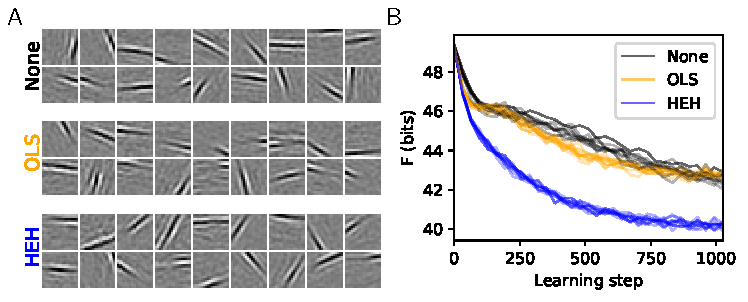
\includegraphics[width=\linewidth]{figure_map}}
%\vspace*{-.1cm}
\caption{
{\bf Role of homeostasis in learning sparse representations}:
We show the results of Sparse Hebbian Learning using different homeostasis algorithms at convergence ($1024$ learning epochs). The compared algorithms are : \texttt{None} (using a simple simple normalization of the atoms), \texttt{OLS} (the method of~\citep{Olshausen97}), \texttt{HEH} (using the optimal homeostasis described in this paper). {\sf (A)}~For each algorithm, we show $18$ atoms from the $441$ filters of the same size as the image patches ($M= 22 \times 22=484$, circularly masked) and presented in a matrix (separated by a white border). The upper and lower row respectively show the least and most probably selected atoms. This highlights the fact that without proper homeostasis, dictionary learning leads to inhomogeneous representations. {\sf (B)}~Evolution of cost  $F$ (in bits, see~\seeEq{L0_cost_full}) as a function of the number of iterations and cross-validated over $10$ runs. While \texttt{OLS} provides a similar convergence than  \texttt{None}, the \texttt{HEH}  method provides a better final convergence.%
\label{fig:map}}%
\end{figure*}%
%%------------------------------%
%: free-energy formulation
% TODO: better define p_\phi and q_\psi / we do a Gaussian mixture models 
Visual items composing natural images are often sparse, such that knowing a model for the generation of images, the brain may use this property to reconstruct images using only a few of these items.
In the context of the representation of natural images\footnote{We use image patches drawn from large images of outdoor scenes, as provided in the \emph{kodakdb} database which is available in the project's repository. %These are circularly masked to avoid artifacts (see Annex 2.3).
} represented in a matrix $\image = (\image_k)_{k=1}^K \in \RR^{K \times M}$ as a set of $K$ vector samples (herein, we will use a batch size of $K=256$) as images raveled along $M$ pixels (each $\image_{k, j} \in \RR$ are the corresponding luminance values), let us assume the generic Generative Linear Model, such that for any sample $k$ the image was generated as $\image_k = \dico^T \coef_{k} + \epsilon $, where by definition, the $N$ coefficients are denoted by $\coef_{k} = (\coef_{k, i})_{i=1}^N \in \RR^{N}$ and the dictionary by $\dico \in \RR^{N \times M}$. Finally, $\epsilon \in \RR^{M}$ is a Gaussian iid noise which is Normal without loss of generality by scaling the norm of the dictionary's rows. Knowing this model, unsupervised learning aims at finding the least surprising causes (the parameters $\hat{\coef}_{k}$ and $\dico$) for the data $\image_k$.
%This should take into account the fact that we may only have access to a (possibly wrong) recognition model $q_\Psi(\coef_{k} | \image_k)$ for any sample $k$ (where $\Psi$ are the parameters of this model) to encode the image into coefficients. In probabilistic term, this amounts to minimize the free-energy $F$ as a bound on surprise of the (unknown) density of the parameters $p_\dico( \coef_{k} | \image_k)$~\citep{Friston12,Kingma13,Doersch2016}:
%TODO: cherish a rigorous argumentation
%\begin{equation} -\log p_\dico( \coef_{k} | \image_k) \leq F \eqdef KL( q_\Psi(\coef_{k} | \image_k) || p_\dico( \coef_{k} | \image_k) )  -\log p_\dico( \coef_{k} | \image_k) \end{equation}
%where the first term in the right hand side is the (positive) Kullback-Leibler distance between the density of images using the current estimate of the (unknown) marginal posterior probability. %
%An advantage of this formulation is that the free-energy can be rewritten as
%\begin{equation} F = KL( q_\Psi(\coef_{k} | \image_k) || p_\dico(\coef_{k}) ) - \int \log p_\dico(\image_k | \coef_{k} ) dq_\Psi(\coef_{k} | \image_k) \end{equation}
%In particular, using a known coding $\hat{\coef_{k}}$ of the image $\image_k$ and by ignoring the first term in the right hand side, we may approximate the free-energy as:
In particular, the cost %relative to using a coding $\hat{\coef_{k}}$ of the image $\image_k$ 
may be formalized in a probabilistic terms as~\citep{Olshausen97}:
\begin{align} 
F &\approx \langle - \log [ p(\image_k | \hat{\coef}_{k}, \dico ) p_\dico(\hat{\coef}_{k}) ]\rangle_{k = 1 \ldots K} \\
&= \langle \frac{1}{2} \norm{\image_k - \dico \hat{\coef}_{k}}_2^2 - \log p_\dico(\hat{\coef}_{k})\rangle_{k = 1 \ldots K} \label{eq:sparse_cost} \end{align}
% https://github.com/bicv/Perrinet2015BICV_sparse/blob/master/sparse.tex#L374
Such hypothesis allows to retrieve the cost that is optimized in most of existing models of unsupervised learning. Explicitly, the representation is optimized by minimizing a cost defined on prior assumptions on representation's sparseness, that is on $\log p_\dico( \coef_{k} )$. For instance, learning is accomplished in {\sc SparseNet}~\citep{Olshausen97} by defining a sparse prior probability distribution function for each coefficients in the factorial form $\log p_\dico(\coef_{k}) \sim -\beta \sum_i \log ( 1 + \frac{a_i^2}{\sigma^2} )$ where $\beta$ corresponds to the steepness of the prior and $\sigma$ to its scaling (see Figure 13.2 from~\citep{Olshausen02}). Then, knowing this sparse solution, learning is defined as slowly changing the dictionary using Hebbian learning.
Indeed, to compute the partial derivative of $F$ with respect to $\dico$, we have $\forall i$:
\begin{align} 
\frac{\partial }{\partial \dico_i } F &= \langle\frac{1}{2} \frac{\partial }{\partial \dico_i }[(\image_k - \dico^T \hat{\coef}_{k})^T (\image_k - \dico^T \hat{\coef}_{k})]\rangle_{k = 1 \ldots K} \\
&= \langle\hat{\coef}_{k} (\image_k - \dico^T \hat{\coef}_{k})\rangle_{k = 1 \ldots K}.
\end{align}
This allows to define unsupervised learning as the (stochastic) gradient descent using this equation. Similarly to Eq.~17 in~\citep{Olshausen97} or to Eq.~2 in~\citep{Smith06}, the relation is a linear ``Hebbian'' rule~\citep{Hebb49} since it enhances the weight of neurons proportionally to the activity (coefficients) between pre- and post-synaptic neurons. Note that there is no learning for non-activated coefficients and also that we used a (classical) scheduling of the learning rate and a proper initialization of the weights (see Annex 2.5 \& 2.6). The novelty of this formulation compared to other linear Hebbian learning rule such as~\citep{Oja82} is to take advantage of the sparse (non-linear) representation, hence the name Sparse Hebbian Learning (SHL).
%It is linear (at the single neuraon level) but the sparse code is not linear (at population level) \textendash link with back-propagation
In general, the parameterization of the prior in~\seeEq{sparse_cost} has major impacts on results of the sparse coding and thus on the emergence of edge-like receptive fields and requires proper tuning. For instance, a L2-norm penalty term (that is, a Gaussian prior on the coefficients) corresponds to Tikhonov regularization~\citep{Tikhonov77} and a L1-norm term (that is, an exponential prior for the coefficients) corresponds to the LASSO convex cost which may optimized by least-angle regression (LARS)~\citep{efron2004least} or FISTA~\citep{beck2009fast}. %In fact, the definition of the prior corresponds to an objective sparseness and does not always fit to the observed probability distribution function of the coefficients.
%This is the classical formulation from~\citet{Olshausen97} but thanks to the free-energy formulation,  we have highlighted here the different hypothesis and approximation made to derive the learning rule.
% In particular the objective is only valid at convergence when the recognition model matches the true prior distribution of coefficients (that is, when $KL( q_\Psi(\coef_{k} | \image_k) || p_\dico(\coef_{k}) )=0$) and this approximation may influence the predicted optimal representation obtained at convergence and which follows the iterations of the learning process.%- a nice move would be to use free-energy as a bound on surprise - and that homeostasis comes as a additional mechanism - restricts the set of possible dictionaries. (for a review, see~\citep{Pece02}) such as numerical optimization~\citep{Olshausen97}, non-negative matrix factorization~\citep{Lee99,Ranzato07} or Matching Pursuit~\citep{Perrinet03ieee,Smith06,Rehn07,Perrinet10shl}
%link of sparse coding with the cortical architecture (see rao and ballard) :
%~~~~~~~~~~~~~~~~~~~~~~~~~~~~~~~~~~~%
\subsection{Algorithm: Sparse Coding with a control mechanism for the selection of atoms}
%~~~~~~~~~~~~~~~~~~~~~~~~~~~~~~~~~~~%
Concerning the choice of a proper prior distribution, the spiking nature of neural information demonstrates that the transition from an inactive to an active state is far more significant at the coding time scale than smooth changes of the firing rate. This is for instance perfectly illustrated by the binary nature of the neural code in the auditory cortex of rats~\citep{DeWeese03}. Binary codes also emerge as optimal neural codes for rapid signal transmission~\citep{Bethge03}. This is also relevant for neuromorphic systems which transmit discrete, asynchronous events (such as a network packet). With a binary event-based code, the cost is only incremented when a new neuron gets active, regardless to its (analog) value. Stating that an active neuron carries a bounded amount of information of $\lambda$ bits, an upper bound for the representation cost of neural activity on the receiver end is proportional to the count of active neurons, that is, to the $\ell_0$ pseudo-norm $\norm{\coef_{k}}_0 = \abs{\enscond{i}{\coef_{k, i} \neq 0}}$:%
% TODO clarify the benefit of using the free energy F
\begin{align}%
F \approx   \langle \frac{1}{2} \norm{\image_k - \dico \coef_{k}}_2^2 + \lambda\norm{\coef_{k}}_0 \rangle_{k = 1 \ldots K}%
\label{eq:L0_cost}%
\end{align}%
This cost is similar with information criteria such as the Akaike Information Criteria~\citep{Akaike74} or distortion rate~\cite[p.~571]{Mallat98}. For $\lambda=\log_2 N$, it gives the total information (in bits) to code for the residual (using entropic coding) and the list of spikes' addresses. In general, the high inter-connectivity of neurons (on average approximately $10000$ synapses per neurons) justifies such an informational perspective with respect to the analog quantization of information in the point-to-point transfer of information between neurons.
However, \seeEq{L0_cost} defines a harder cost to optimize (in comparison to convex formulations in Equation~\ref{eq:sparse_cost} for instance) since the hard $\ell_0$ pseudo-norm sparseness leads to a non-convex optimization problem which is \emph{NP-complete} with respect to the dimension $M$ of the dictionary~\cite[p.~418]{Mallat98}.
%The different SHL algorithms simply differ by the coding step.
%This implies that they only differ by first, how sparseness is defined at a functional level and second, how the inverse problem corresponding to the coding step is solved at the algorithmic level.
%Most of the schemes cited above use a less strict, parametric definition of sparseness (like the convex L$_1$-norm), but for which a mathematical formulation of the optimization problem exists.
%Few studies such as~\citep{Liu14,Peharz12} use the stricter $\ell_0$ pseudo-norm as the coding problem gets more difficult.
%A thorough comparison of these different strategies was recently presented in~\citep{Charles12}.
%See also~\citep{Aharon06} for properties of the coding solutions to the $\ell_0$ pseudo-norm.
%Similarly, in~\citep{Perrinet10shl}, we preferred to retrieve an approximate solution to the coding problem to have a better match with the measure of efficiency~\seeEq{L0_cost}. % (see Section~\ref{sec:matchingpursuit} for a description of the algorithm)

Still, there are many solutions to this optimization problem and here, we will use a generalized version of the {\color{red}Matching} {\color{olive}Pursuit} (MP) algorithm~\cite[p.~422]{Mallat98}. A crucial aspect of this algorithm is the $\ArgMax$ function as it produces at each step a competition among $N$ neurons (that is, $\lambda$ bits). For this reason, we will introduce a mechanism to tune this competition. For any signal $\image_k$ drawn from the database, we get the coefficients $\coef_{k} = S(\image_k; \Psi=\{\dico, z, N_0\})$ thanks to the sparse coding step. The parameter $N_0>0$ controls the amount of sparsity that we impose to the coding. The novelty of this generalization of MP lies in the scalar functions $z = \{z_i \}_{i = 1 \ldots N }$ which control the competition for the best {\color{red}match} across atoms. While an identical symmetric function is chosen in the original MP algorithm (that is, $\forall i, z_i(\coef_{k}) = |\coef_{k}|$), we will define these at a first attempt as the rescaled non-linear rectified linear unit (ReLU) with gain $\gamma_i$: $\forall i, z_i (\coef_{k,i}) = \gamma_i * \coef_{k,i} * \delta(\coef_{k,i}>0)$ where $\delta$ is Kronecker's indicator function.
%\begin{algorithm}
%\caption{Generalized Matching Pursuit: $\coef_{k} = S(\image_k; \Psi=\{\dico, z, N_0\})$}\label{alg:gmp}
\begin{algorithmic}[1]
\State set the sparse vector $\coef_{k}$ to zero,
\State initialize $\bar{\coef_{k}}_i=\langle\image_k, \dico_i \rangle$ for all $i$
\While{$\norm{\coef_{k}}_0<N_0$}:
\State {\color{red}select the best match: $i^\ast = \ArgMax_{i} [z_i( \bar{\coef_{k}}_i )]$}
\State update the sparse coefficient: $\coef_{k, i^\ast} = \coef_{k, i^\ast} + \bar{\coef_{k, i^\ast}}$,
\State {\color{olive}update residual: $\forall i, \bar{\coef_{k,i}} \leftarrow \bar{\coef_{k,i}} - \coef_{k,i^\ast} \langle\dico_{i^\ast} , \dico_i \rangle $.% for all $i$ using~\seeEq{mp3},
}
\EndWhile
\end{algorithmic}
%\end{algorithm}
%It is at this point important to note that in this algorithm,
%we achieve an exponential convergence of the squared error~\citep[p.~422]{Mallat98},
%but also that this curve can be directly derived from the coefficients' values.
%Indeed, for $N$ coefficients (that is, $\| \coef \|_0 = N$), we have the squared error equal to:
%\begin{equation}%
%E_N \eqdef \| \image - \dico\coef \| ^2 / \| \image \| ^2 = 1 - \sum_{1\leq k\leq N} a_{k}^2 / \| \image \| ^2%
%\label{eq:error}%
%\end{equation}%
%As a consequence, the sparser the distributions of coefficients, then quicker is the decrease of the residual energy.
%%Note that the observed distribution of coefficients follow a power-law. This was already observed in~\citep{Perrinet03ieee}. This power-law (``scale-free'') distribution is defined by
%%\begin{equation}%
%%\log p(a) \propto - \zeta \log a_{k}%
%%\label{eq:powerlaw}%
%%\end{equation}%
%%The value of $\zeta$ quantifies therefore the strength of the sparseness in the signal.
%% discuss this? or say it will be discussed below

% method zero = just normalizing the coefficitents (Mairal14)
We found as in~\citep{Rehn07} that by using an algorithm like Matching Pursuit (that is using the symmetric function or setting $\forall i, \gamma_i=1$ as in~\citep{Mairal14} for instance), the Sparse Hebbian Learning algorithm could provide results similar to {\sc SparseNet}. An advantage is the non-parametric assumption on the prior based on this more generic $\ell_0$ pseudo-norm sparseness. However, we observed that this class of algorithms could lead to solutions corresponding to a local minimum of the full objective function: Some solutions seem as efficient as others for representing the signal but do not represent edge-like features homogeneously (\seeFig{map}-A, \texttt{None}). %  With a correct tuning of parameters, we observed that different coding schemes show qualitatively a similar emergence of edge-like filters. The specific coding algorithm used to obtain this sparseness appears to be of secondary importance as long as it is adapted to the data and yields sufficiently efficient sparse representation vectors. However, resulting dictionaries vary qualitatively among these schemes and it was unclear which algorithm is the most efficient and what was the individual role of the different mechanisms that constitute SHL schemes. At the learning level, we have shown that the homeostasis mechanism had a great influence on the qualitative distribution of learned filters~\citep{Perrinet10shl}.~\citep{Perrinet10shl}
Moreover, using other sparse coding algorithms which are implemented in the \verb+sklearn+ library, we compared the convergence of the learning with different sparse coding algorithms. In particular, we compared the learning as implemented with matching pursuit to that with orthogonal matching pursuit (OMP)~\citep{pati1993orthogonal}, LARS or FISTA (see Annex 2.4). %
% TODO answer What do you mean by "some cells learn 'faster'"? This is the justification for your homeostatis mechanism but it is not shown in your paper. Also, I guess you did not provide the annex. The 'Annex.html' document has a section "Testing different algorithms" but it only display 5 algorithms that perform the same, which does not convince me that some extra mechanism is needed.
% show the example in the map / synthetic unbalanced network
For all these sparse coding algorithms, during the early learning step, some cells may learn ``faster'' than others. In particular, these cells have more peaked distributions of their activity and tend to be selected more often. There is the need for a homeostasis mechanism that will ensure convergence of learning. The goal of this work is to study the specific role of homeostasis in learning sparse representations and to propose a homeostasis mechanism based on the functions $z_i$ which optimizes the learning of an efficient representation.%
%~~~~~~~~~~~~~~~~~~~~~~~~~~~~~~~~~~~~~~~~~~~~~~~~~~~~%
\subsection{Algorithm: Histogram Equalization Homeostasis}\label{HEH}
%~~~~~~~~~~~~~~~~~~~~~~~~~~~~~~~~~~~~~~~~~~~~~~~~~~~~%
%------------------------------%
%: see Figure~\ref{fig:HEH}
%: \seeFig{HEH}
\begin{figure*}%[!ht]%[p!]%%
\centering{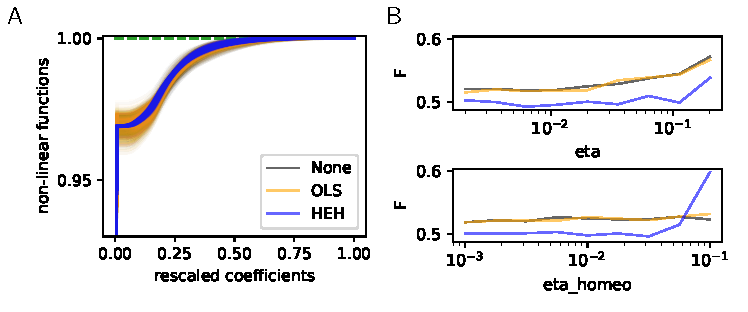
\includegraphics[width=\linewidth]{figure_HEH}}
%\vspace*{-.1cm}
\caption{
{\bf Histogram Equalization Homeostasis and its role in unsupervised learning}:
{\sf (A)}~Non-linear homeostatic functions $z_i, \forall i$ learned using Hebbian learning. These functions were computed for different homeostatic strategies (\texttt{None}, \texttt{OLS} or \texttt{HEH}) but only used in \texttt{HEH}. Note that for our choice of $N_0=13$, all cumulative functions start around $1 - N_0/N \approx .970 $. At convergence of \texttt{HEH}, the probability of choosing any filter is equiprobable, while the distribution of coefficients is more variable for \texttt{None} and \texttt{OLS}. As a consequence, the distortion between the distributions of sparse coefficients is minimal for \texttt{HEH}, a property which is essential for the optimal representation of signals in distributed networks such as the brain. %
{\sf (B)}~Effect of learning rate $\eta$ (\texttt{eta}) and homeostatic learning rate $\eta_h$ (\texttt{eta\_homeo}) on the final cost as computed for the same learning algorithms but with different homeostatic strategies (\texttt{None}, \texttt{OLS} or \texttt{HEH}). Parameters were explored around a default value, on a logarithmic scale and over 4 octaves. This shows that \texttt{HEH} is robust across a wide range of parameters.
%We show the results of Sparse Coding using the two different homeostasis algorithms using surrogate data where each filter was equiprobable but for which we manipulated the first half of the coefficients to be artificially twice as big. %
%{\sf (A)}~Such a situation replicates a situation arising during learning when a sub-group of filters is more active, e.~g. because it learned more salient features. Here, we show the probability of the selection of the different filters (normalized to an average of $1$) which shows a bias of the standard Matching Pursuit to select more often filters whose activity is higher. %We evaluated the efficiency of retrieving the correct coefficients to about $\ %
%{\sf (B)}~Non-linear homeostatic functions learned using Hebbian learning. These functions were initialized as the cumulative distribution function of uniform random variables. Then they are used to modify choices in the Matching step of the Matching Pursuit algorithm. Progressively, the non-linear functions converge to the (hidden) cumulative distributions of the coefficients of the surrogate, clearly showing the group of filters with twice a big coefficients.
% {\sf (C)}~At convergence, the probability of choosing any filter is uniform. As a result, entropy is maximal, a property which is essential for the optimal representation of signals in distributed networks such as the brain.
\label{fig:HEH}}%
\end{figure*}%
%------------------------------%
% TODO Say explictly that we reproduce ~\citep{Perrinet10shl} + python code
% - a measure is that the Orientation Selectivity (OS) is highest - because we know that the structure of the world is like this...
% - goals = memory / separation / representation
% we know that during learning, there are distortions in the code / dictionary : normalisation is not enough.
Knowing a dictionary and a sparse coding algorithm, we may transform any data sample $\image_k$ into a set of sparse coefficients using the above algorithm: $\coef_{k} = S(\image_k; \Psi=\{\dico, z, N_0\})$. In particular, at any step \emph{during} learning, dictionaries may not have been homogeneously learned and may exhibit different distributions. %But in general, this operation may be also feasible for any other representation dictionary.  
However, this would not be taken into account in the original cost (see~\seeEq{L0_cost}) as we assumed as in~\cite{Olshausen97} that $p_\dico(\hat{\coef_{k}})$ is factorized, that is, that the components of the sparse vector are independent. As a consequence, we may use a deviation to this hypothesis as an additional component to the cost: 
\begin{equation}%
F \approx  \langle \frac{1}{2} \norm{\image_k - \dico \coef_{k}}_2^2 + \lambda\norm{\coef_{k}}_0 + \texttt{MI}(\coef_{k}) \rangle_{k = 1 \ldots K}%
\label{eq:L0_cost_full}%
\end{equation}%
Where we used the mutual information $\texttt{MI}$ as a proxy to measure the dependence between the components of the sparse vector. %
%As we have seen above, a component of the free-energy is $KL( q_\Psi(\coef_{k} | \image_k) || p_\dico(\coef_{k}) )$ which decreases over a set of samples if and only if the recognition model gets closer to the true generative model. 
%As we have seen above, a component of the free-energy is $KL( q_\Psi(\coef_{k} | \image_k) || p_\dico(\coef_{k}) )$ which decreases over a set of samples if and only if the recognition model gets closer to the true generative model. 
%While the latter is hidden, we know about its structure in an optimal representation within a population of sensory neurons. 
Indeed, as information is coded in the address of neurons, information transfer as computed through Shannon entropy, is optimized when the activity within the neural population is uniformly balanced, that is when each neuron is \emph{a priori} selected with the same probability. In particular, a necessary (yet not sufficient) condition for minimizing this cost is that the prior probability of selecting coefficients are identical $\forall (i,j), q_\Psi(\coef_{k,i})=q_\Psi(\coef_{k,j})$ to ensure the optimality of the choice of the $\ell_0$ pseudo-norm and compare it to the representation in the primary visual cortex. As we have seen, we may use different transformation functions $z_i$ to influence the choice of coefficients such that we may use these functions to optimize the objective cost defined by~\seeEq{L0_cost_full}. 
% mutual information $KL( q_\Psi(\coef | \image_k) \leq MI( q_\Psi(\coef)$%

%: % using cumulative distribution = "inverse transform sampling" / circular problem= has to be done progressively
% a monotonic point scalar function does not change the KL distance / free-energy
To achieve this uniformity, we may define an homeostatic gain control mechanism based on histogram equalization, that is, by transforming coefficients in terms of quantiles by setting $\forall i, z_i(\cdot) = P( \cdot > a_i)$. Such a transform is similar to the inverse transform sampling which is used to optimize representation in auto-encoders~\citep{Doersch2016} and can be considered as a non-parametric extension of the ``re-normalization trick'' used in variational auto-encoders~\citep{Kingma13}. %
Moreover, it has been found that such an adaptation mechanism is observed in the response of the retina to various contrast distributions~\citep{Laughlin81}. However, an important point to note is that this joint optimization problem between coding and homeostasis is circular as we can not access the true posterior $p_\dico(\coef)$: Indeed, the coefficients depend on non-linear coefficients through $\coef_{k} = S(\image_k; \Psi=\{\dico, z_i, N_0\})$, while the non-linear functions depend on the (cumulative) distribution of the coefficients. We will make the assumption that such a problem can be solved iteratively by slowly learning the non-linear functions. Starting with an initial set of non-linear functions as in \texttt{None}, we will derive an approximation for the sparse coefficients. Then, the function $z_i$ for each coefficient of the sparse vector is calculated using an iterative moving average scheme (parameterized by time constant $1/\eta_h$) to smooth its evolution during learning. At the coding level, this non-linear function is incorporated in the matching step of the matching pursuit algorithm, to modulate the choice of the most probable as that corresponding to the maximal quantile: $i^\ast = \ArgMax_i z_i(a_i)$. We will coin this variant as Histogram Equalization Homeostasis (\texttt{HEH}). The rest of this Sparse Hebbian Learning algorithm is left unchanged. As we adapt the dictionaries progressively during Sparse Hebbian Learning, we may incorporate this \texttt{HEH} homeostasis during learning by choosing an appropriate learning rate $\eta_h$.
To recapitulate the different choices we made from the learning to the coding and the homeostasis, the unsupervised learning can be summarized using the following steps:
%The proposed algorithm is:
%\begin{algorithm}
%\caption{Homeostatic Unsupervised Learning of Kernels:  $\dico = H(\image; \eta, \eta_h, N_0)$}\label{alg:shl}
\begin{algorithmic}[1]
\State Initialize the point non-linear gain functions $z_i$ to similar cumulative distribution functions,%
\State initialize atoms $\dico_i$ to random points on the $K$-unit sphere,
\For{$T$ epochs}: % TODO : use a convergence criterium instead
\State draw a new batch  $\image$ from the database of natural images,%
\For{ each data point $\image_k$}: % TODO : use a convergence criterium instead
\State  compute the sparse representation vector using sparse coding $\coef = S(\image_k; \Psi=\{\dico, z, N_0\})$,
% TODO use momentum?  ~\citep{Mairal2010}
\State modify atoms: $\forall i, \dico_{i} \leftarrow \dico_{i} + \eta \cdot \coef_{i} \cdot (\image_k - \dico \coef)$,% using~\seeEq{learn},
\State normalize atoms: $\forall i, \dico_{i} \leftarrow \dico_{i} / \norm{\dico_{i}}$,% using~\seeEq{learn},
\State {\color{blue} update homeostasis functions: $\forall i, z_i( \cdot ) \leftarrow (1- \eta_h ) \cdot z_i( \cdot ) + \eta_h \cdot \delta( a_i \leq \cdot)$.% using~\seeEq{learn_homeo}
}
\EndFor
\EndFor
\end{algorithmic}
%\end{algorithm}
%
%\begin{enumerate}%
%\item Initialize the point non-linear gain functions $z_i$ to similar cumulative distribution functions and the atoms $\dico_i$ to random points on the unit $K$-dimensional sphere,%
%\item repeat until learning converged:%
%\begin{enumerate}
%\item draw a signal $\image_k$ from the database,%
%\item compute sparse representation vector $\coef = S(\image_k; \Psi=\{\dico, z_i, N0\})$
%\item modify dictionary: $\forall i, \dico_{i} \leftarrow \dico_{i} + \eta a_{i} (\image_k - \dico\coef)$,% using~\seeEq{learn},
%\item normalize dictionary: $\dico_{i} \leftarrow \dico_{i} / \norm{\dico_{i}}$,% using~\seeEq{learn},
%{\color{MidnightBlue}
%\item update homeostasis functions: $z_i( \cdot ) \leftarrow (1- \eta_h ) z_i( \cdot ) + \eta_h \delta( a_i \leq \cdot)$.% using~\seeEq{learn_homeo}
%}
%\end{enumerate}
%\end{enumerate}

We compared qualitatively the set $\dico$ of receptive filters generated with different homeostasis algorithms (see Fig.~\ref{fig:map}-A). A more quantitative study of the coding is shown by comparing the decrease of the cost as a function of the iteration step (see Fig.~\ref{fig:map}-B). This demonstrate that forcing the learning activity to be uniformly spread among all receptive fields results in a faster convergence of the representation error as represented by the decrease of the cost $F$. %
%----------------------------------------------------------------------------%
\subsection{Results: Fast unsupervised learning using homeostasis}\label{results}
%----------------------------------------------------------------------------%
%%------------------------------%
% TODO:  this rule does not seem to improve the results when compared to pre-existing rule such as EMP (Figure3). The quantitative evaluation of this rule is also not sufficient as the different results are only evaluated in term of optimization cost and do not appear to be evaluated on a test set.
%: \seeFig{HAP}
\begin{figure*}%[!ht]%[p!]%
\centering{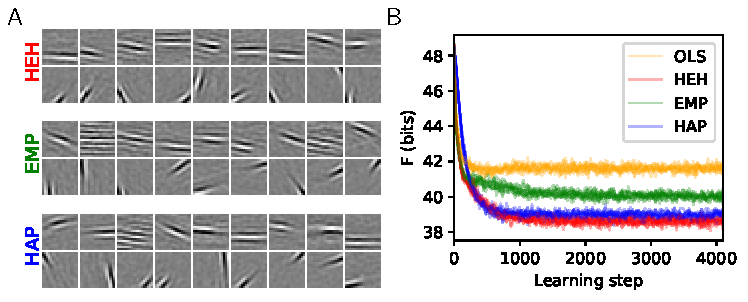
\includegraphics[width=\linewidth]{figure_HAP}}
%\vspace*{-.1cm}
\caption{
{\bf Homeostasis on Activation Probability (\texttt{HAP}) and a quantitative evaluation of homeostatic strategies}: %
 {\sf (A)}~$18$ from the $441$ dictionaries learned for the two heuristics \texttt{EMP} and \texttt{HAP} and compared to the optimal homeostasis (see \seeFig{map}-A, \texttt{HEH}).
 Again, the upper and lower row respectively show the least and most probably selected atoms.  {\sf (B)}~Comparison of the cost $F$ during learning and cross-validated over $10$ runs: The convergence of \texttt{OLS} is similar to \texttt{EMP}. The simpler \texttt{HAP} heuristics gets closer to the more demanding \texttt{HEH} homeostatic rule, demonstrating that this heuristic is a good compromise for fast unsupervised learning.
\label{fig:HAP}}%# TODO: include OLS
%\caption{
%{\bf Quantitative role of homeostasis in a classification network}: We used the generic MNIST protocol to assess the role of the homeostasis algorithm on classification. %
% {\sf (A-C)}~144 dictionaries learned from the MNIST database with a sparseness of 5 after 10000 iterations with {\sf (A)}~MP Algorithm ($\eta=0.01$): No homeostasis regulation, only a small subset of dictionaries are selected with a high probability to describe the dataset.
%{\sf (B)}~SPARSENET Algorithm ($\eta=0.01$, $\eta_h=0.01$, $\alpha_h=0.02$): The homeostasis regulation is made by normalizing the volatility.
%{\sf (C)}~MEUL Algorithm ($\eta=0.01$, $\eta_h=0.01$): All dictionaries are selected with the same probability to describe the dataset, leading to a cooperative learning.
% {\sf (D)}~Comparison of the reconstruction error (computed as the square root of the squared difference between the image and the residual) for the 3 algorithms (MEUL, SPARSENET, MP): The convergence velocity of MEUL is higher than SPARSENET and MP.
%\label{fig:quant}}%
\end{figure*}%
%%------------------------------%
%\subsection{Algorithm: Approximate homeostasis}\label{HAP}
%: incompatible with nueromimetic / fast implementation
%- first method = Olshausen's homeostasis that is a gradient descent on the variance of coefficients. serves as a control
% (\seeFig{map}-A, \texttt{OLS})
We have shown above that we can find an exact solution to the problem of homeostasis during Sparse Hebbian Learning. However, this solution has several drawbacks. First, it is computationally intensive on a conventional computer as it necessitates to store each $z_i$ function to store the cumulative distribution of each coefficient. More importantly, it seems that biological neurons seem to rather use a simple gain control mechanism. This can be implemented by modifying the gain $\gamma_i$ of the slope of the ReLu function to operate a gradient descent on the cost based on the distribution of each coefficients. Such strategy can be included in the SHL algorithm by replacing line 8 in the learning lgorithm. For instance, the strategy of~\citep{Olshausen97} assumes a cost on the difference between the observed variance of coefficients $V_i$ as computed over a set of samples compared to a desired value $\sigma_g^2$ (and assuming a multiplicative noise parameterized by $\alpha$) :
\begin{align}
&V_i \leftarrow (1- \eta_h ) \cdot V_i + \eta_h \cdot 1/K\sum_{k=1\cdots K} a_{i, k}^2 \\ &\textrm{ and }
\gamma_i \leftarrow \gamma_i \cdot \left( \frac{V_i}{\sigma_g^2} \right)^\alpha
\end{align}%
This is similar to the mechanisms of gain normalization proposed by~\cite{Schwartz01} and which were recently shown to provide efficient coding mechanisms by~\cite{Simoncelli17}. However, compared to these methods which manipulate the gain of dictionaries based on the energy of coefficients, we propose to rather use a methodology based on the probability of activation. Indeed, the main distortion that occurs during learning is on higher statistical moments rather than variance, for instance when an atom is winning more frequently during the earliest iterations, its pdf will typically be more kurtotic than a filter that has learned less.
%TODO say that in these variants this replaces 2e in the learning

%: Comparison to Sandin
Recently, such an approach was proposed by~\cite{Sandin17}. Based on the same observations, the authors propose to optimize the coding during learning by modulating the gain of each dictionary element based on the recent activation history. They base their Equalitarian Matching Pursuit (\texttt{EMP}) algorithm on a heuristics which cancels the activation of any filter that was more often activated than a given threshold probability (parameterized by $1+\alpha_h$). In our setting, we may compute a similar algorithm using an evaluation of probability of activation followed by binary gates:
\begin{align}%
&p_i \leftarrow (1- \eta_h ) \cdot p_i + \eta_h \cdot 1/K\sum_{k=1\cdots K} \delta(a_{i, k} > 0) \\ &\textrm{ and }
\gamma_i = \delta (p_i < N_0/N*(1+\alpha_h) )
\end{align}%
Interestingly, they reported that such a simple heuristic could improve the learning, deriving a similar result as we have shown in~\seeFig{map} and~\seeFig{HEH}. %Moreover they have shown that such a homeostatic mechanism is more important than optimizing the coding algorithm, for instance by using OMP instead of MP.
Again, such strategy can be included in line 8 of the learning algorithm.

%: derivation
% TODO: - HAP: The proposed approximation HAP is the novelty of this paper, as it permits to reduce the computational cost of the HEH technique with an approximate regularizing function z_i. However, the construction of this rule is not detailed enough. It is introduced as modulation change needed to maximize the entropy of the coefficient activation probability but this part should be extended to give more insight on such construction.
Similarly, we may derive an approximate homeostasis algorithm based on the current activation probability but using a gradient descent approach on gain modulation. Ideally, this corresponds to finding $\gamma_i$ such that we minimize the entropy $-\sum_{i=1\cdots N} p_i \log p_i$. However, the sparse coding function $S(\image_k; \Psi=\{\dico, z, N_0\})$ is not differentiable. %, yet we may use the expression of the cumulative probability functions to see the quantitative effect of $\gamma_i$ on activation probability. 
One possible heuristic is then to differentiate the change of modulation gain that would be necessary to achieve an equiprobable probability, that is when $\forall i, p_i = p_0 \eqdef N_0 / N$: % this replaces step 2 e in the learning
%      # cf. https://github.com/VictorBoutin/CHAMP/blob/caa2a77cc65d0043db1aeb11eedb707633a93df4/CHAMP/CHAMP_Layer.py#L365
%      gain = np.exp(-(1 / alpha_homeo) * (mean_measure-target))
\begin{align}%
&p_i \leftarrow (1- \eta_h ) \cdot p_i + \eta_h \cdot 1/K\sum_{k=1\cdots K} \delta(a_{i, k} > 0) \\ &\textrm{ and }
\gamma_i = \exp(-(p_i - p_0) / \alpha_h)
\end{align}%
We will coin this variant of the algorithm Homeostasis on Activation Probability (\texttt{HAP}). % derivation p.56N de 2018-01-09 HULK
%\subsection{Approximate homeostasis yields similar performance}
Following these derivations, we quantitatively compared \texttt{OLS}, \texttt{EMP} and \texttt{HAP} to \texttt{HEH} (see~\seeFig{HAP}). This shows that while \texttt{EMP} slightly outperforms \texttt{OLS} (which itself is more efficient than \texttt{None}, see~\seeFig{HEH}-B), \texttt{HAP} proves to be closer to the optimal solution given by \texttt{HEH}. %
% effect of coding algorithm
In particular, we replicated in \texttt{HAP} the result of~\cite{Sandin17} that while homeostasis was essential in improving unsupervised learning, the coding algorithm (MP versus OMP) mattered relatively little (see Annex 2.4). Also, we verified the dependence of this efficiency with respect to different hyperparameters (as we did in~\seeFig{HEH}-B). %
Overall, these quantitative results show that the~\texttt{HEH} algorithm could be replaced by a simpler and more rapid heuristic, \texttt{HAP}, which is based on activation probability. This would generate similar efficiency for the coding of patches from natural images.
%-----------------------------------------------------------------%
\section{Discussion and conclusion}\label{discussion-et-conclusion}
%-----------------------------------------------------------------%
%%------------------------------%
%: \seeFig{CNN}
\begin{figure*}[!ht]%[p!]%
\centering{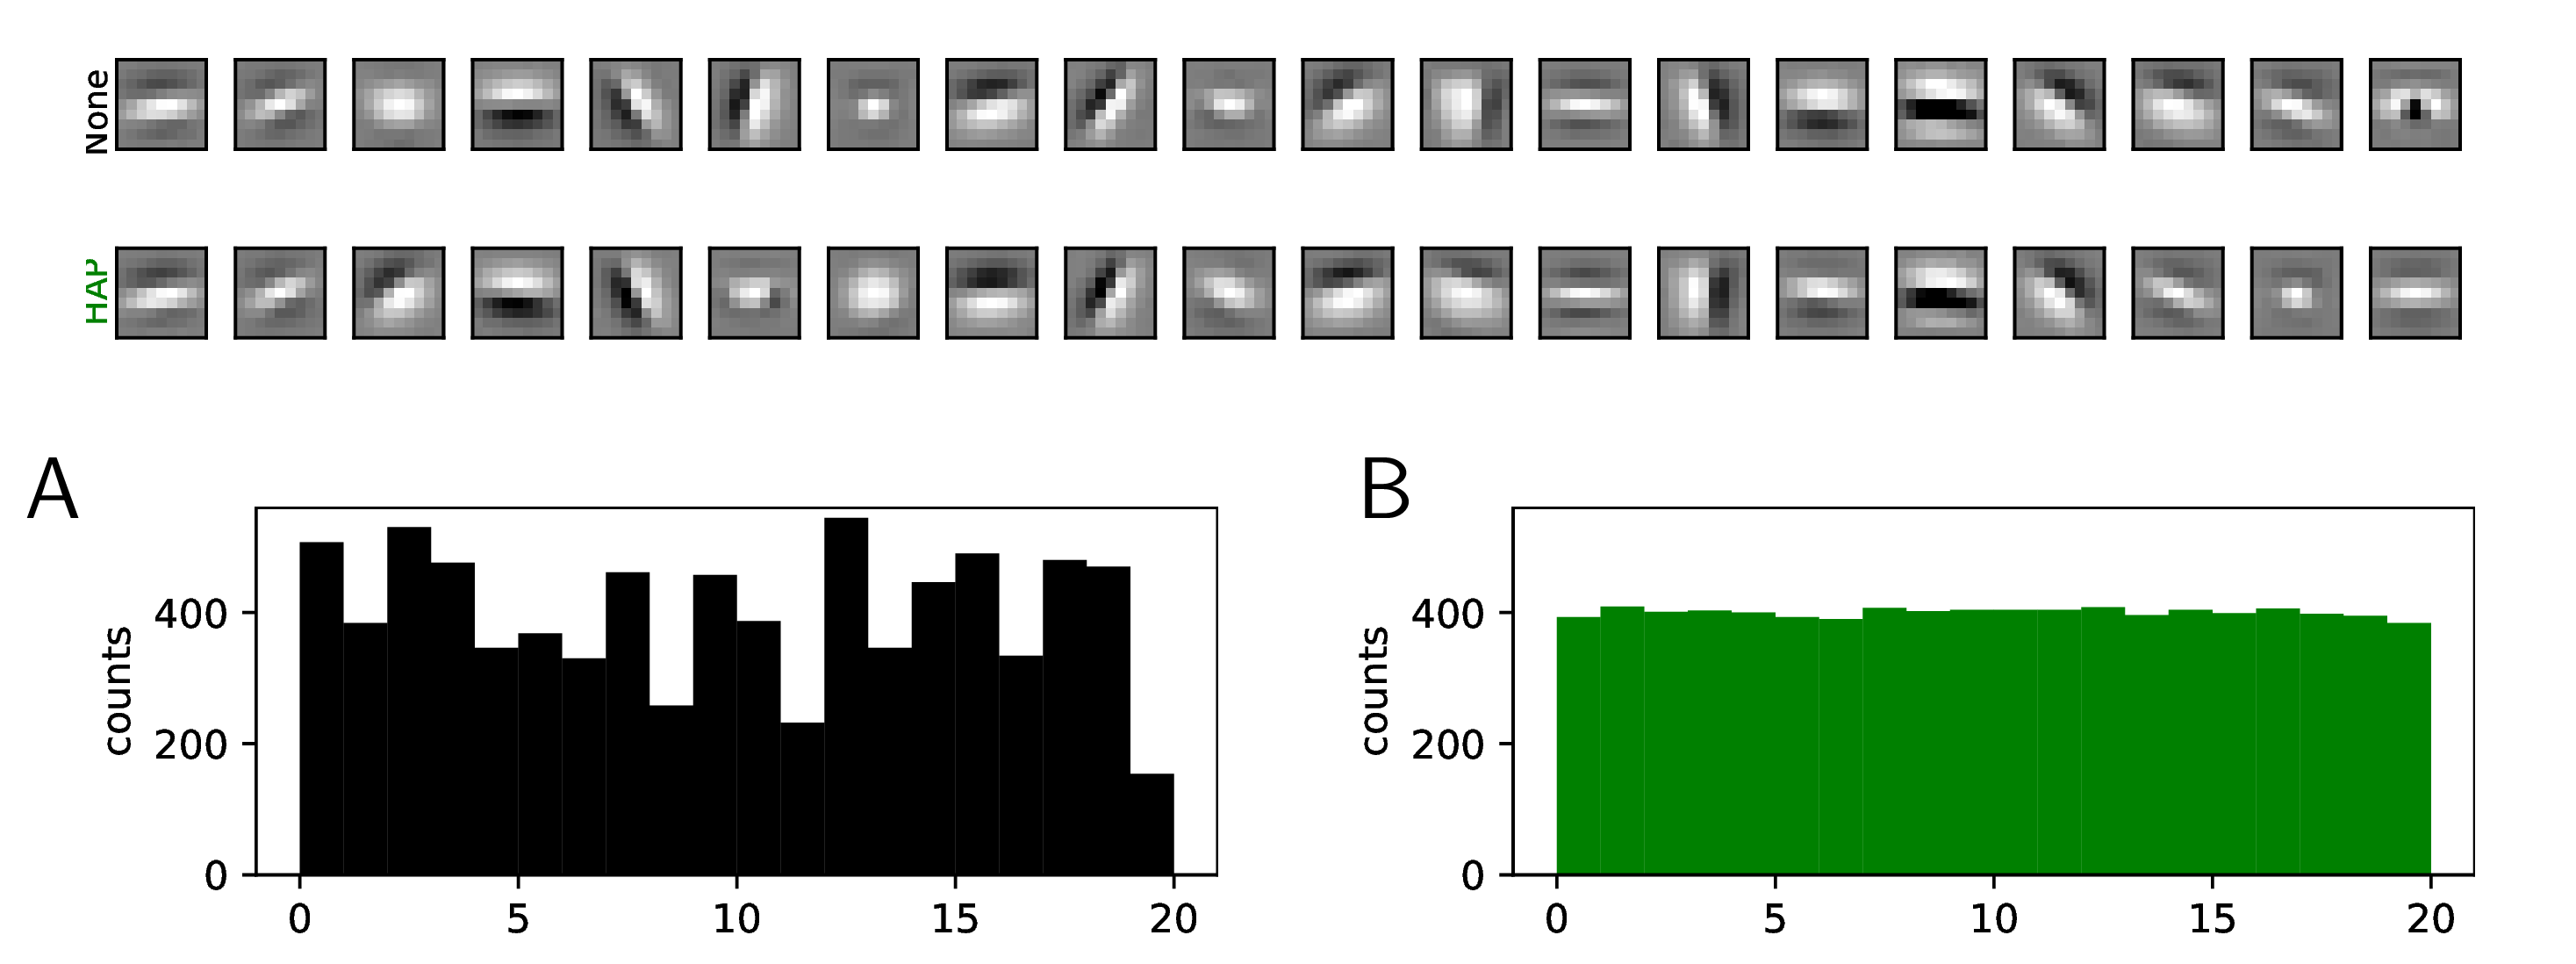
\includegraphics[width=\linewidth]{figure_CNN}}
%\vspace*{-.1cm}
\caption{
{\bf Extension to Convolutional Neural Networks (CNNs)}: %
 We extend the HAP algorithm to a single layered CNN with $20$ kernels and using the ATT face database. We show here the kernels learned without (\texttt{None}, top row) and with (\texttt{HAP}, bottom row) homeostasis (note that we used the same initial conditions). As for the simpler case, we observe a heterogeneity of activation counts without homeostasis, that is, in the case which simply normalizes the energy of kernels (see {\sf (A)}). With homeostasis, we observe the convergence of the activation probability for the different kernels (see {\sf (B)}). This demonstrates that this heuristic extends well to a CNN architecture.
\label{fig:CNN}}%# TODO: do figure :-0
\end{figure*}%
%%------------------------------%
%: 2- benchmarking of computation time: toward event-driven?
% Finally, we show that such an algorithm can be extended to convolutional architectures and we show the results obtained on different natural image databases.
One core advantage of sparse representations is the efficient coding of complex signals using compact codes. Inputs are thus represented as combination of few elements drawn from a large dictionary of atoms. As a consequence, a common design for unsupervised learning rules relies on a gradient descent over a cost measuring representation quality with respect to sparseness. This constraint introduces a competition between atoms. In the context of the efficient processing of natural images, we proposed here that such strategies can be optimized by including a proper homeostatic regulation enforcing a fair competition between the elements of the dictionary. We implemented this rule by introducing a non-linear gain normalization similar to what is observed in biological neural networks. We validated this theoretical insight by challenging this adaptive unsupervised learning algorithm with different heuristics for the homeostasis. Simulations show that at convergence, while the coding accuracy did not vary much, including homeostasis changed qualitatively the learned features. In particular, homeostasis results in a more homogeneous set of orientation selective filters, which is closer to what is found in the visual cortex of mammals~\citep{Ringach02,Rehn07,Loxley17}. To further validate these results, we quantitatively compared the efficiency of the different variants of the algorithms, both at the level of homeostasis (homeostatic learning rate, parameters of the heuristics), but also to the coding (by changing $M$, $N$ or $N_0$) and to the learning (by changing the learning rate, the scheduling or $M$). This demonstrated that overall, this neuro-inspired homeostatic algorithm provided with the best compromise between efficiency and computational cost. 

%2. importance of homeo - vanishing term in deep learning -> use deep learning to validate output
%3. application to asynchronous / focal log-polar (retinal) input / continuous learning / credit assignement (no access to true residual)
In summary, this biologically-inspired learning rule demonstrates that principles observed in neural computations can help improve real-life machine learning algorithms. Indeed, by developing this fast learning algorithm, we hope for its use in artificial intelligence algorithms. This type of architecture is economical, efficient and fast. In particular the HAP algorithms uses only ReLUs such that it is easy to be transferred to most deep learning algorithms.  %In particular, we are considering perspectives for coding within a dynamic flow of sensory data and we hope to apply this type of algorithm on embedded systems such as aerial robots. 
Along with this, we hope that this new type of rapid unsupervised learning algorithm can provide a normative theory for the coding of information in low-level sensory processing, whether it is visual or auditory, for example. Moreover, by its nature, this algorithm can easily be extended to convolutional networks such as those used in deep learning neural networks. This extension is possible by extending the filter dictionary by the hypothesis of invariances to the translation of representations. Our results on different databases show the stable and rapid emergence of characteristic filters on these different bases (see \seeFig{CNN} and Annex 3.1). This result shows a probable prospect of extending this representation and for which we hope to obtain classification results superior to the algorithms existing in the state-of-the-art. As such, empirical evaluations of the proposed algorithms should be extended. For instance, it would be very useful to test for image classification results on standard benchmark datasets. %Finally such computational results highlight the importance of homeostasis in unsupervised learning algorithms and for the study of neural systems.
% HAP what limits?
% theorems.
% another perspective is precision-weighted inference see page 11 of Kingma
%%%%%-----------------------------------------------------------------
%\section*{Acknowledgments}
%\Acknowledgments
%%%-----------------------------------------------------------------
%\printbibliography
%\bibliographystyle{IEEEtran}
%\bibliography{hulk}
% Generated by IEEEtran.bst, version: 1.12 (2007/01/11)
\begin{thebibliography}{10}
\providecommand{\url}[1]{#1}
\csname url@samestyle\endcsname
\providecommand{\newblock}{\relax}
\providecommand{\bibinfo}[2]{#2}
\providecommand{\BIBentrySTDinterwordspacing}{\spaceskip=0pt\relax}
\providecommand{\BIBentryALTinterwordstretchfactor}{4}
\providecommand{\BIBentryALTinterwordspacing}{\spaceskip=\fontdimen2\font plus
\BIBentryALTinterwordstretchfactor\fontdimen3\font minus
  \fontdimen4\font\relax}
\providecommand{\BIBforeignlanguage}[2]{{%
\expandafter\ifx\csname l@#1\endcsname\relax
\typeout{** WARNING: IEEEtran.bst: No hyphenation pattern has been}%
\typeout{** loaded for the language `#1'. Using the pattern for}%
\typeout{** the default language instead.}%
\else
\language=\csname l@#1\endcsname
\fi
#2}}
\providecommand{\BIBdecl}{\relax}
\BIBdecl

\bibitem{Hubel68}
\BIBentryALTinterwordspacing
D.~H. Hubel and T.~N. Wiesel, ``Receptive fields and functional architecture of
  monkey striate cortex.'' \emph{Journal of {P}hysiology}, vol. 195, no.~1, pp.
  215--243, Mar. 1968. [Online]. Available:
%  \url{http://www.ncbi.nlm.nih.gov/pmc/articles/PMC1557912/}
\BIBentrySTDinterwordspacing

\bibitem{Olshausen96}
\BIBentryALTinterwordspacing
B.~A. Olshausen and D.~J. Field, ``Natural image statistics and efficient
  coding,'' \emph{Network: {C}omputation in {N}eural {S}ystems}, vol.~7, no.
  6583, pp. 333--9, Jun. 1996. [Online]. Available:
%  \url{http://dx.doi.org/10.1038/381607a0}
\BIBentrySTDinterwordspacing

\bibitem{Vincent08}
P.~Vincent, H.~Larochelle, Y.~Bengio, and P.-A. Manzagol, ``Extracting and
  composing robust features with denoising autoencoders,'' in \emph{Proceedings
  of the 25th international conference on Machine learning}.\hskip 1em plus
  0.5em minus 0.4em\relax ACM, 2008, pp. 1096--1103.

\bibitem{Sulam2017multi}
J.~Sulam, V.~Papyan, Y.~Romano, and M.~Elad, ``Multi-layer convolutional sparse
  modeling: Pursuit and dictionary learning,'' \emph{arXiv preprint
  arXiv:1708.08705}, 2017.

\bibitem{MakhzaniF13}
\BIBentryALTinterwordspacing
A.~Makhzani and B.~J. Frey, ``k-sparse autoencoders,'' \emph{CoRR}, vol.
  abs/1312.5663, 2013. [Online]. Available:
%  \url{http://arxiv.org/abs/1312.5663}
\BIBentrySTDinterwordspacing

\bibitem{Papyan16}
V.~Papyan, Y.~Romano, and M.~Elad, ``Convolutional neural networks analyzed via
  convolutional sparse coding,'' \emph{stat}, vol. 1050, p.~27, 2016.

\bibitem{Kingma13}
D.~P. {Kingma} and M.~{Welling}, ``{Auto-Encoding Variational Bayes},''
  \emph{ArXiv e-prints}, Dec. 2013.

\bibitem{Olshausen97}
\BIBentryALTinterwordspacing
B.~A. Olshausen and D.~J. Field, ``Sparse coding with an overcomplete basis
  set: A strategy employed by {V1}?'' \emph{Vision Research}, vol.~37, no.~23,
  pp. 3311--3325, Dec. 1997. [Online]. Available:
%  \url{http://dx.doi.org/10.1016/S0042-6989(97)00169-7}
\BIBentrySTDinterwordspacing

\bibitem{Mairal14}
J.~Mairal, F.~Bach, J.~Ponce \emph{et~al.}, ``Sparse modeling for image and
  vision processing,'' \emph{Foundations and Trends in Computer Graphics and
  Vision}, vol.~8, no. 2-3, pp. 85--283, 2014.

\bibitem{Marder2006variability}
E.~Marder and J.-M. Goaillard, ``Variability, compensation and homeostasis in
  neuron and network function,'' \emph{Nature Reviews Neuroscience}, vol.~7,
  no.~7, p. 563, 2006.

\bibitem{Hansel12}
D.~Hansel and C.~van Vreeswijk, ``The mechanism of orientation selectivity in
  primary visual cortex without a functional map,'' \emph{Journal of
  Neuroscience}, vol.~32, no.~12, pp. 4049--4064, 2012.

\bibitem{Schwartz01}
O.~Schwartz and E.~P. Simoncelli, ``Natural signal statistics and sensory gain
  control,'' \emph{Nature Neuroscience}, vol.~4, no.~8, pp. 819--25, 2001.

\bibitem{Carandini12}
\BIBentryALTinterwordspacing
M.~Carandini and D.~J.~D. Heeger, ``Normalization as a canonical neural
  computation,'' \emph{Nature Reviews Neuroscience}, vol.~13, no. November, pp.
  1--12, jan 2012. [Online]. Available:
  \url{http://discovery.ucl.ac.uk/1332718/
  http://www.ncbi.nlm.nih.gov/pubmed/22108672
  http://www.pubmedcentral.nih.gov/articlerender.fcgi?artid=PMC3273486}
\BIBentrySTDinterwordspacing

\bibitem{Ringach02}
D.~L. Ringach, ``Spatial structure and symmetry of simple-cell receptive fields
  in macaque primary visual cortex,'' \emph{Journal of neurophysiology},
  vol.~88, no.~1, pp. 455--463, 2002.

\bibitem{Rehn07}
M.~Rehn and F.~T. Sommer, ``A model that uses few active neurones to code
  visual input predicts the diverse shapes of cortical receptive fields,''
  \emph{Journal of {C}omputational {N}euroscience}, vol.~22, no.~2, pp.
  135--46, 2007.

\bibitem{Loxley17}
\BIBentryALTinterwordspacing
P.~N. Loxley, ``The two-dimensional gabor function adapted to natural image
  statistics: A model of simple-cell receptive fields and sparse structure in
  images,'' \emph{Neural Computation}, vol.~29, no.~10, pp. 2769--2799, oct
  2017. [Online]. Available: \url{http://www.ncbi.nlm.nih.gov/pubmed/28777727
  http://www.mitpressjournals.org/doi/abs/10.1162/neco_a_00997}
\BIBentrySTDinterwordspacing

\bibitem{Brito16}
C.~S. Brito and W.~Gerstner, ``Nonlinear hebbian learning as a unifying
  principle in receptive field formation,'' \emph{PLoS computational biology},
  vol.~12, no.~9, p. e1005070, 2016.

\bibitem{Rao99}
\BIBentryALTinterwordspacing
R.~Rao and D.~Ballard, ``Predictive coding in the visual cortex: a functional
  interpretation of some extra-classical receptive-field effects,''
  \emph{Nature {N}euroscience}, vol.~2, no.~1, pp. 79--87, Jan. 1999. [Online].
  Available: \url{http://dx.doi.org/10.1038/4580}
\BIBentrySTDinterwordspacing

\bibitem{Perrinet10shl}
\BIBentryALTinterwordspacing
L.~U. Perrinet, ``Role of homeostasis in learning sparse representations,''
  \emph{Neural Computation}, vol.~22, no.~7, pp. 1812--1836, Jul. 2010.
  [Online]. Available:
  \url{http://invibe.net/LaurentPerrinet/Publications/Perrinet10shl}
\BIBentrySTDinterwordspacing

\bibitem{Sandin17}
\BIBentryALTinterwordspacing
F.~Sandin and S.~Martin-del Campo, ``Dictionary learning with equiprobable
  matching pursuit,'' \emph{arXiv preprint arXiv:1611.09333}, pp. 557--564, may
  2017. [Online]. Available: \url{http://ieeexplore.ieee.org/document/7965902/}
\BIBentrySTDinterwordspacing

\bibitem{Olshausen02}
B.~A. Olshausen, ``Sparse codes and spikes,'' in \emph{Probabilistic {M}odels
  of the {B}rain: {P}erception and {N}eural {F}unction}, R.~P.~N. Rao, B.~A.
  Olshausen, and M.~S. Lewicki, Eds.\hskip 1em plus 0.5em minus 0.4em\relax MIT
  Press, 2002, ch. Sparse Codes and Spikes, pp. 257--72.

\bibitem{Smith06}
\BIBentryALTinterwordspacing
E.~C. Smith and M.~S. Lewicki, ``Efficient auditory coding,'' \emph{Nature},
  vol. 439, no. 7079, pp. 978--982, Feb. 2006. [Online]. Available:
  \url{http://dx.doi.org/10.1038/nature04485}
\BIBentrySTDinterwordspacing

\bibitem{Hebb49}
D.~O. Hebb, \emph{The organization of behavior: {A} neuropsychological
  theory}.\hskip 1em plus 0.5em minus 0.4em\relax New York: Wiley, 1949.

\bibitem{Oja82}
E.~Oja, ``A {S}implified {N}euron {M}odel as a {P}rincipal {C}omponent
  {A}nalyzer,'' \emph{Journal of {M}athematical biology}, vol.~15, pp. 267--73,
  1982.

\bibitem{Tikhonov77}
\BIBentryALTinterwordspacing
A.~N. Tikhonov, \emph{Solutions of {Ill-Posed} Problems}.\hskip 1em plus 0.5em
  minus 0.4em\relax Washington: Winston \& Sons, 1977. [Online]. Available:
  \url{http://www.amazon.com/exec/obidos/redirect?tag=citeulike07-20\&path=ASIN/0470991240}
\BIBentrySTDinterwordspacing

\bibitem{efron2004least}
B.~Efron, T.~Hastie, I.~Johnstone, R.~Tibshirani \emph{et~al.}, ``Least angle
  regression,'' \emph{The Annals of statistics}, vol.~32, no.~2, pp. 407--499,
  2004.

\bibitem{beck2009fast}
A.~Beck and M.~Teboulle, ``A fast iterative shrinkage-thresholding algorithm
  for linear inverse problems,'' \emph{SIAM journal on imaging sciences},
  vol.~2, no.~1, pp. 183--202, 2009.

\bibitem{DeWeese03}
\BIBentryALTinterwordspacing
M.~R. DeWeese, M.~Wehr, and A.~M. Zador, ``Binary spiking in auditory cortex,''
  \emph{Journal of Neuroscience}, vol.~23, no.~21, pp. 7940--7949, Aug. 2003.
  [Online]. Available:
  \url{http://www.jneurosci.org/content/23/21/7940.abstract}
\BIBentrySTDinterwordspacing

\bibitem{Bethge03}
M.~Bethge, D.~Rotermund, and K.~Pawelzik, ``Second order phase transition in
  neural rate coding: Binary encoding is optimal for rapid signal
  transmission,'' \emph{Physical {R}eview {L}etters}, vol.~90, no.~8, p.
  088104, 2003.

\bibitem{Akaike74}
H.~Akaike, ``A new look at the statistical model identification,'' \emph{I{EEE}
  Transactions on Automatic Control}, vol.~19, pp. 716--23, 1974.

\bibitem{Mallat98}
S.~Mallat, \emph{A wavelet tour of signal processing}, 2nd~ed.\hskip 1em plus
  0.5em minus 0.4em\relax Academic Press, 1998.

\bibitem{pati1993orthogonal}
Y.~C. Pati, R.~Rezaiifar, and P.~S. Krishnaprasad, ``Orthogonal matching
  pursuit: Recursive function approximation with applications to wavelet
  decomposition,'' in \emph{Signals, Systems and Computers, 1993. 1993
  Conference Record of The Twenty-Seventh Asilomar Conference on}.\hskip 1em
  plus 0.5em minus 0.4em\relax IEEE, 1993, pp. 40--44.

\bibitem{Doersch2016}
\BIBentryALTinterwordspacing
C.~Doersch, ``Tutorial on variational autoencoders,'' \emph{arXiv:1606.05908
  [cs, stat]}, Jun. 2016. [Online]. Available:
  \url{http://arxiv.org/abs/1606.05908}
\BIBentrySTDinterwordspacing

\bibitem{Laughlin81}
\BIBentryALTinterwordspacing
S.~Laughlin, ``A simple coding procedure enhances a neuron's information
  capacity.'' \emph{Zeitschrift f\"{u}r Naturforschung. Section C:
  Biosciences}, vol.~36, no. 9-10, pp. 910--912, 1981. [Online]. Available:
  \url{http://view.ncbi.nlm.nih.gov/pubmed/7303823}
\BIBentrySTDinterwordspacing

\bibitem{Simoncelli17}
E.~P. Simoncelli, ``Optimal representations and efficient coding,''
  \emph{Annual Review of Vision Science}, vol.~3, no.~1, 2017.

\end{thebibliography}
%%%-----------------------------------------------------------------
%\newpage
%\pagestyle{empty}
%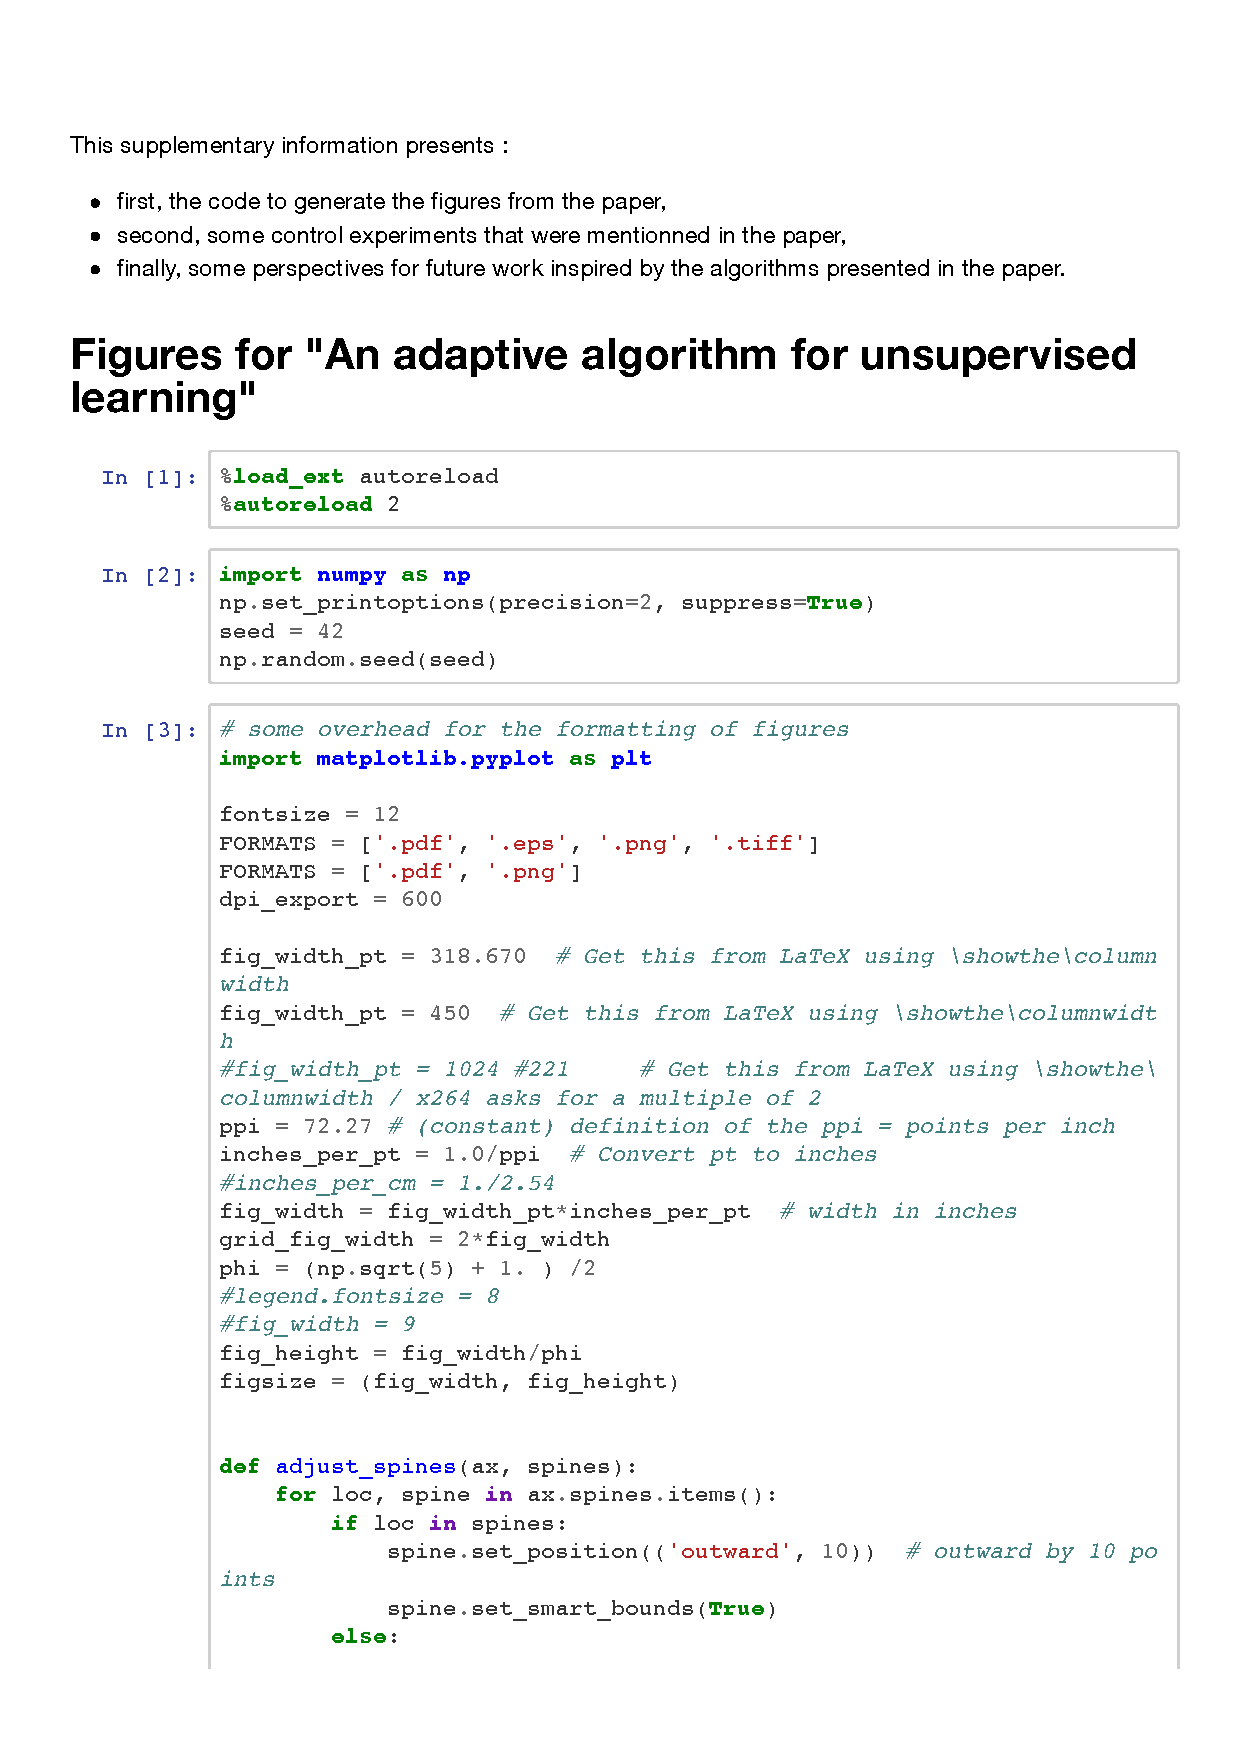
\includepdf[pages=-, fitpaper=true, pagecommand={
%\addcontentsline{toc}{section}{Appendix}},width=\textwidth]{Annex.pdf}
% width=\printingPaperWidth, fitpaper=true, scale=0.25, 
%%%-----------------------------------------------------------------
\end{document}